% !TeX root = ../main.tex
\documentclass[./../main.tex]{subfiles}

\begin{document}

Phần này mô tả sản phẩm cuối sau quá trình phát triển của em, bao gồm
hình ảnh của giao diện người dùng thuộc phần client. Phần giao diện
người dùng sẽ được bạn Phạm Thị Dân mô tả kỹ hơn ở một báo cáo khác.

\subsection{Luồng sử dụng của sinh viên}

\paragraph*{Sinh viên đọc bài đăng}

\begin{itemize}
\item Hình \ref{fig:student_home_page}: Sinh viên truy cập trang chủ và chọn bài đăng muốn đọc.
\item Hình \ref{fig:student_read_post_page}: Giao diện hiển thị bài đăng đã chọn.
\end{itemize}

\begin{figure}[]
	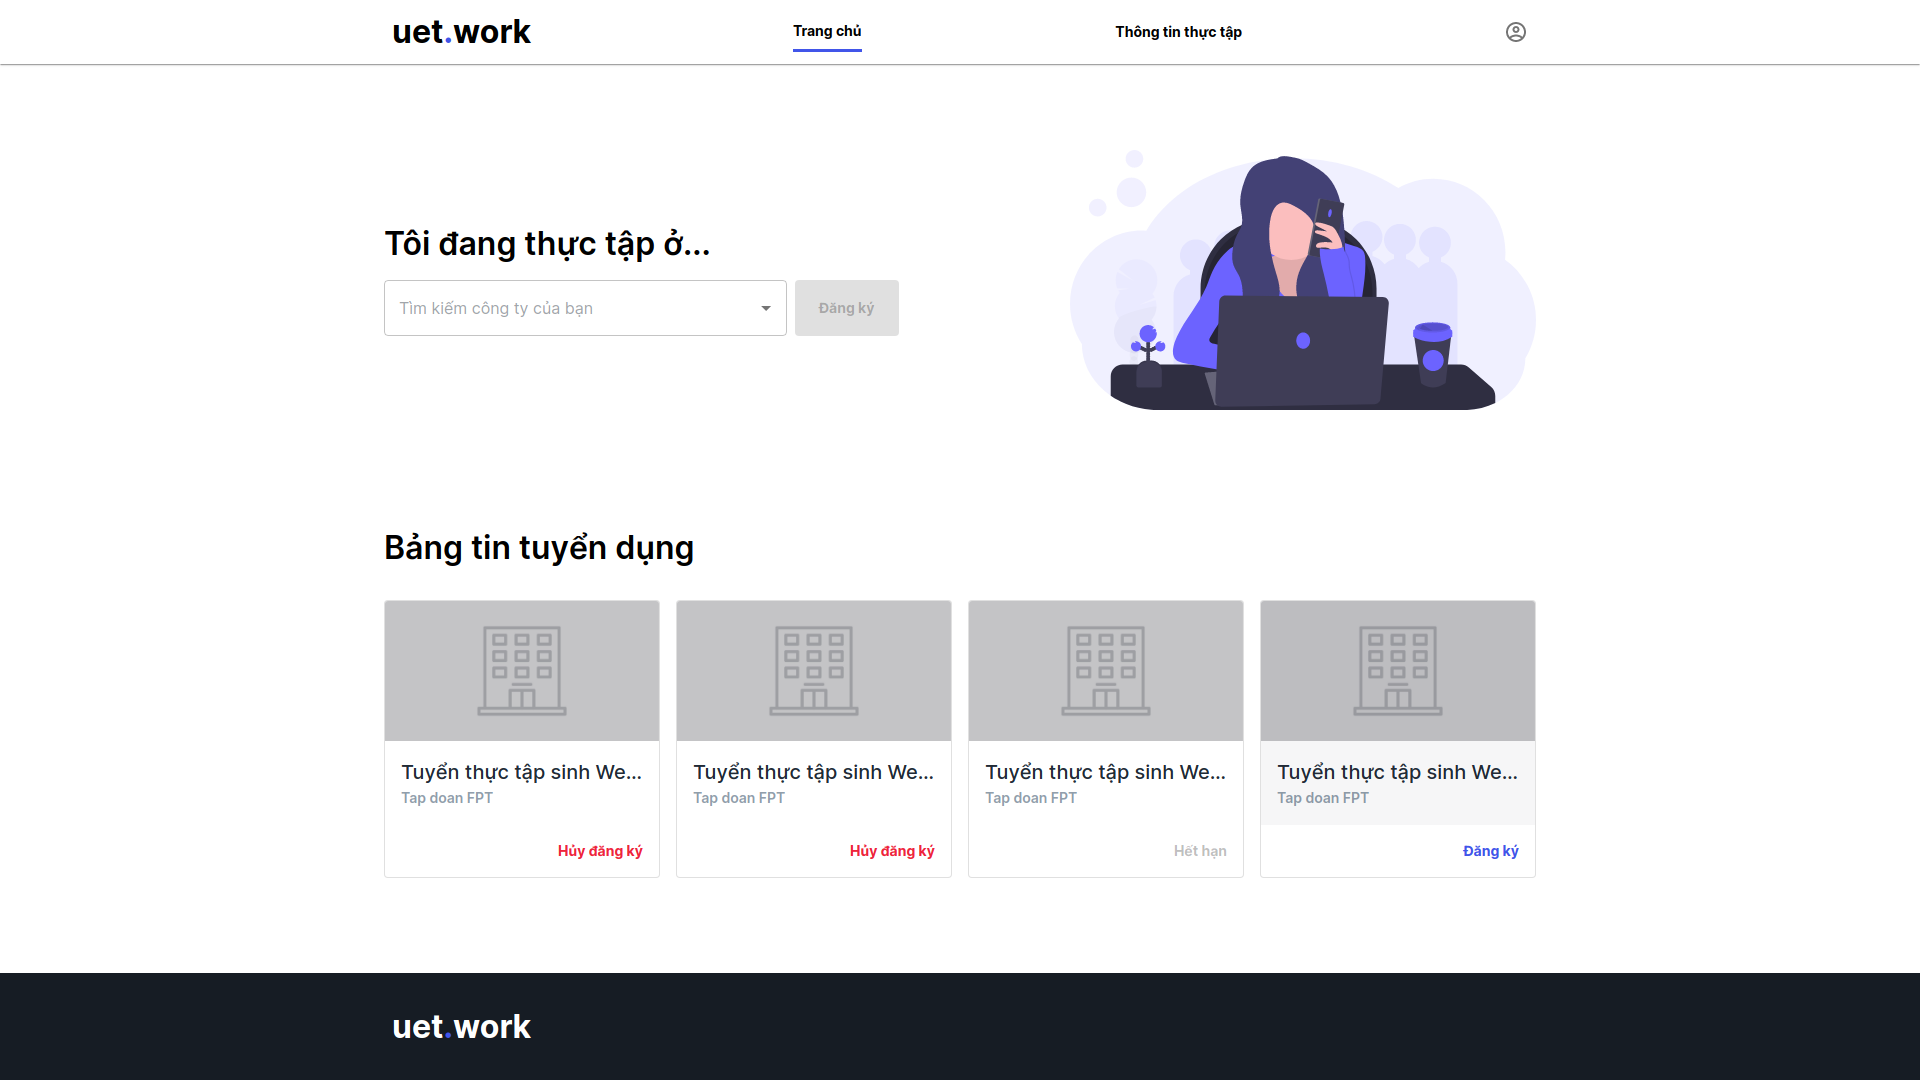
\includegraphics[width=\linewidth]{./images/image37.png}
	\caption{Luồng \emph{Đọc bài đăng}: Truy cập trang chủ và chọn bài đăng muốn đọc}
	\label{fig:student_home_page}
\end{figure}

\begin{figure}[]
	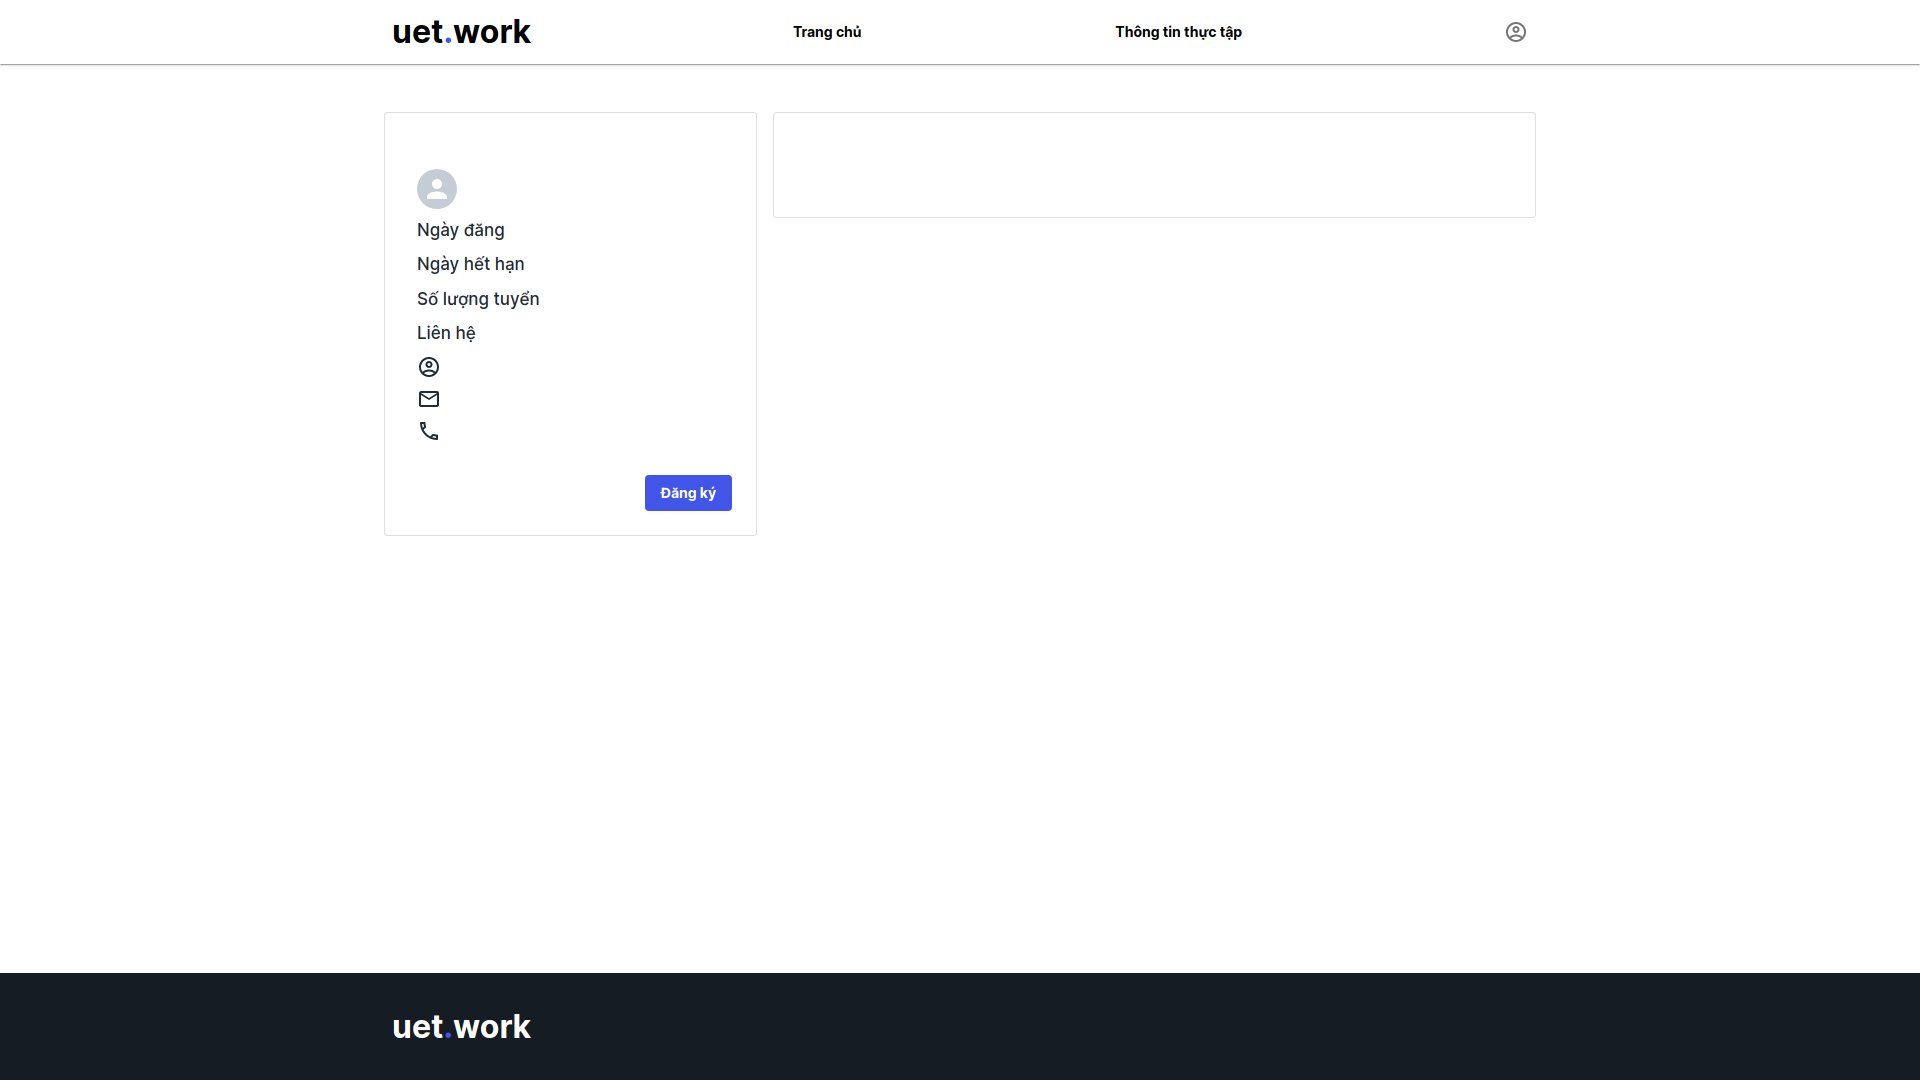
\includegraphics[width=\linewidth]{./images/image38.png} %TODO: replace image
	\caption{Luồng \emph{Đọc bài đăng}: Giao diện hiển thị bài đăng đã chọn}
	\label{fig:student_read_post_page}
\end{figure}

\paragraph*{Sinh viên đăng ký thực tập}

\begin{itemize}
	\item Hình \ref{fig:student_find_company}: Sinh viên tìm kiếm công ty mà mình đang thực tập và đăng ký. 
	\item Hình \ref{fig:student_register_company_success}: Nếuthành công,  hệ thống hiển thị thông báo đăng ký thành công.
	\item Hình \ref{fig:student_register_company_failed}: Nếu thất bại, hệ thống hiển thị thông báo đăng ký thất bại.
\end{itemize}

\begin{figure}[]
	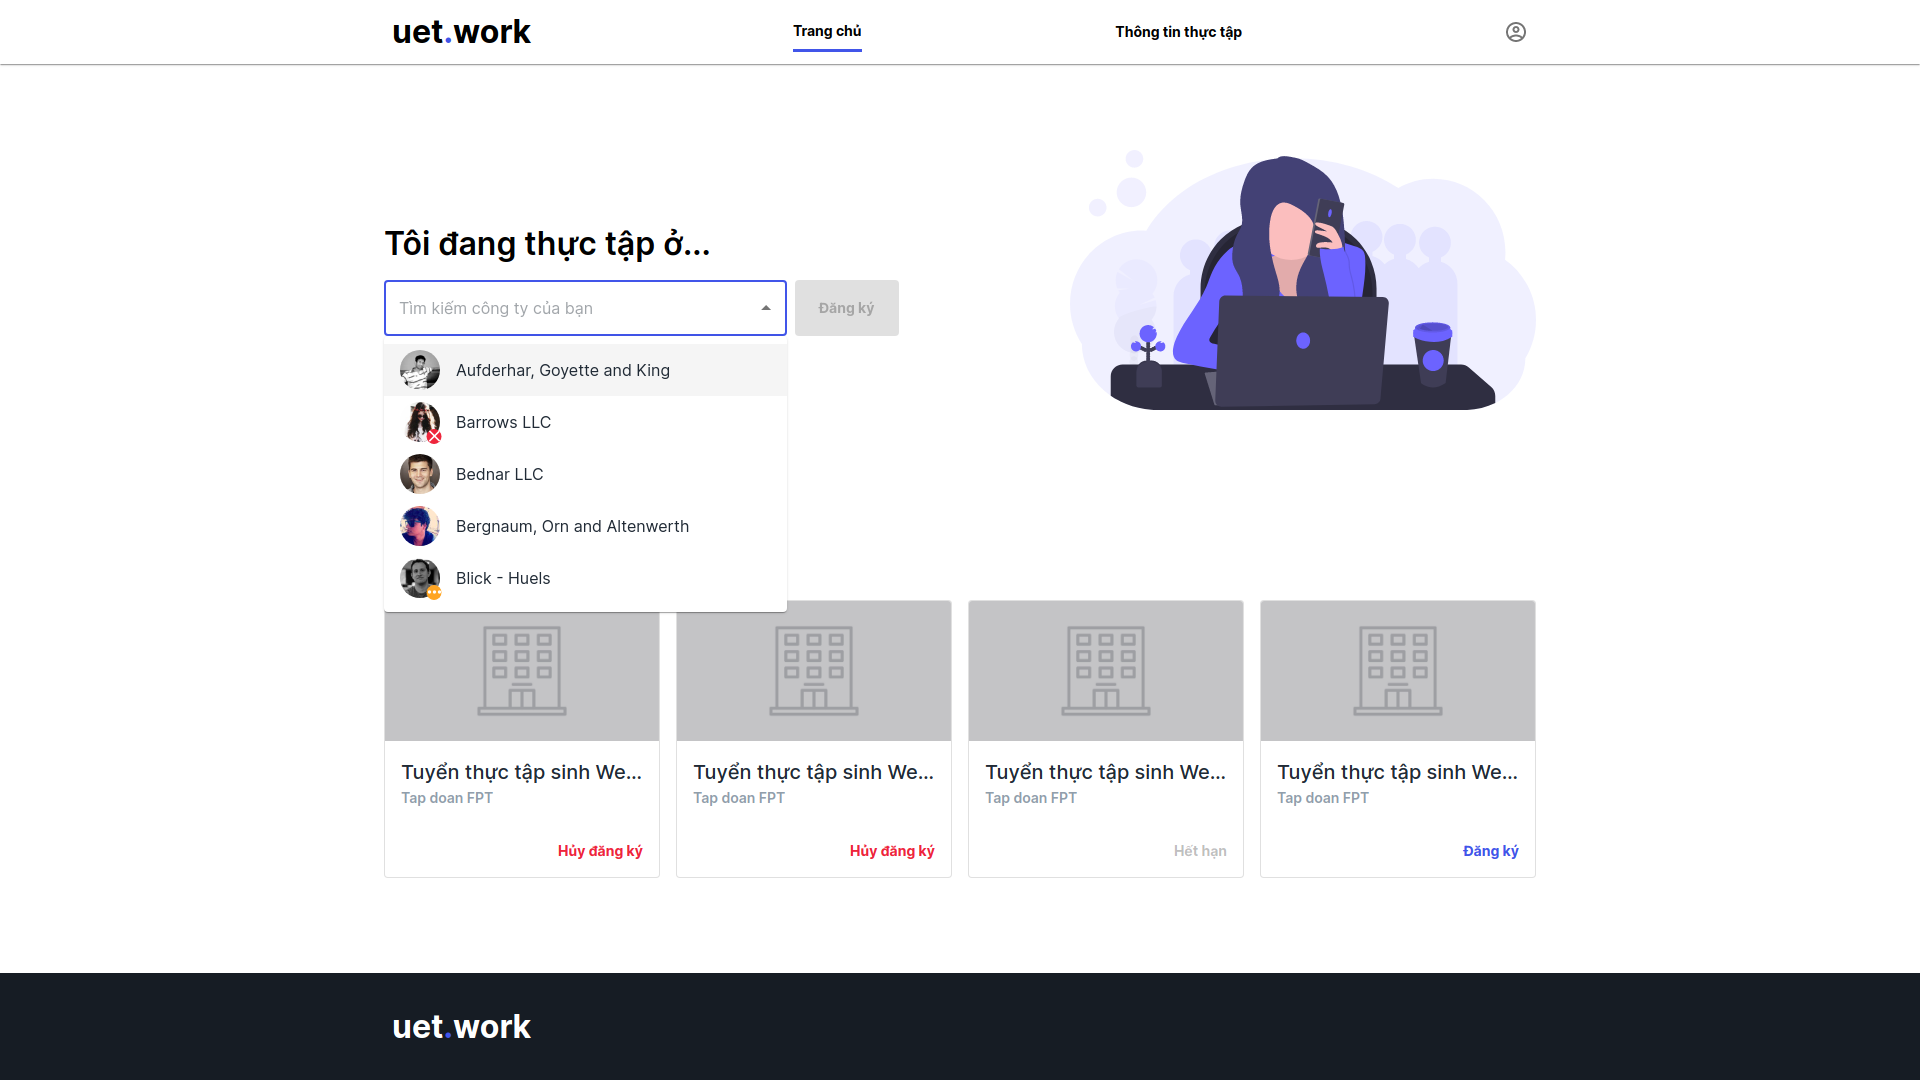
\includegraphics[width=\linewidth]{./images/image39.png}
	\caption{Luồng \emph{Sinh viên đăng ký thực tập}: Tìm kiếm công ty}
	\label{fig:student_find_company}
\end{figure}

\begin{figure}[]
	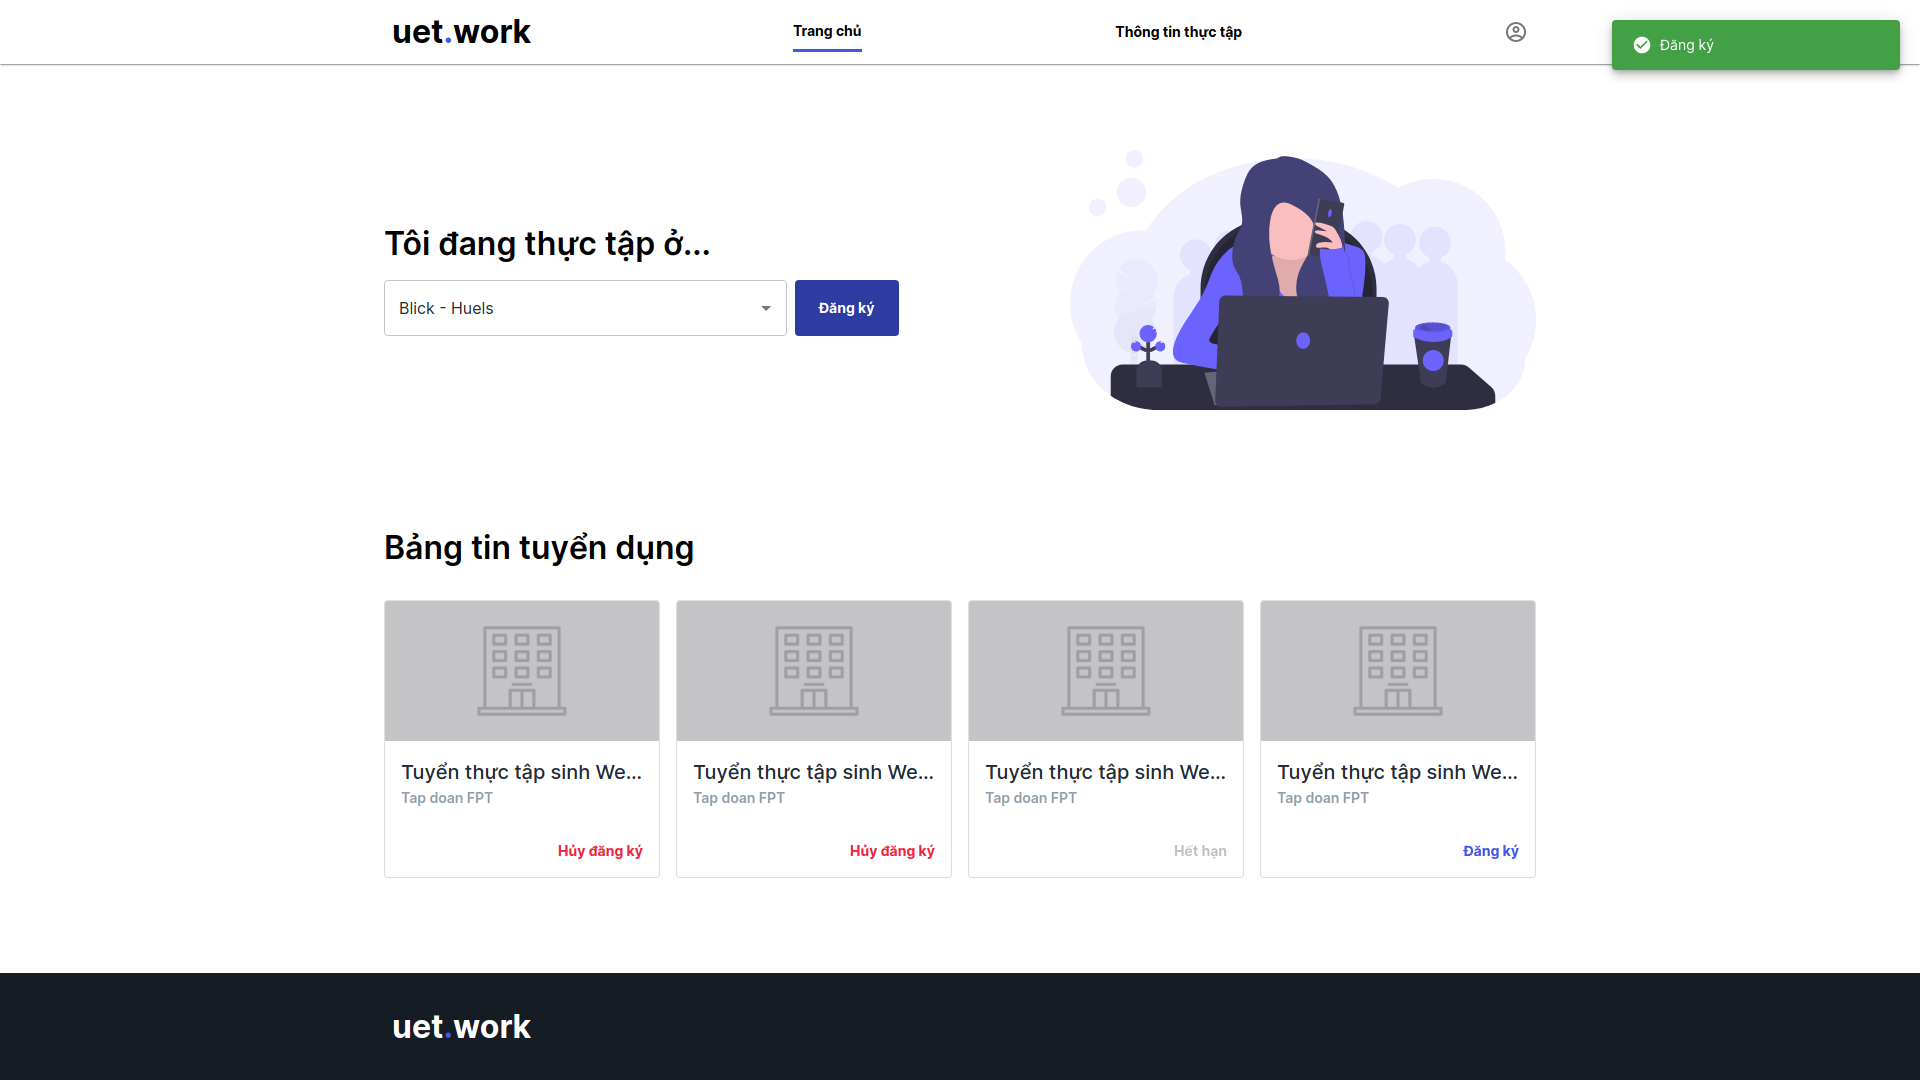
\includegraphics[width=\linewidth]{./images/image40-1.png}
	\caption{Luồng \emph{Sinh viên đăng ký thực tập}: Đăng ký thành công}
	\label{fig:student_register_company_success}
\end{figure}

\begin{figure}[]
	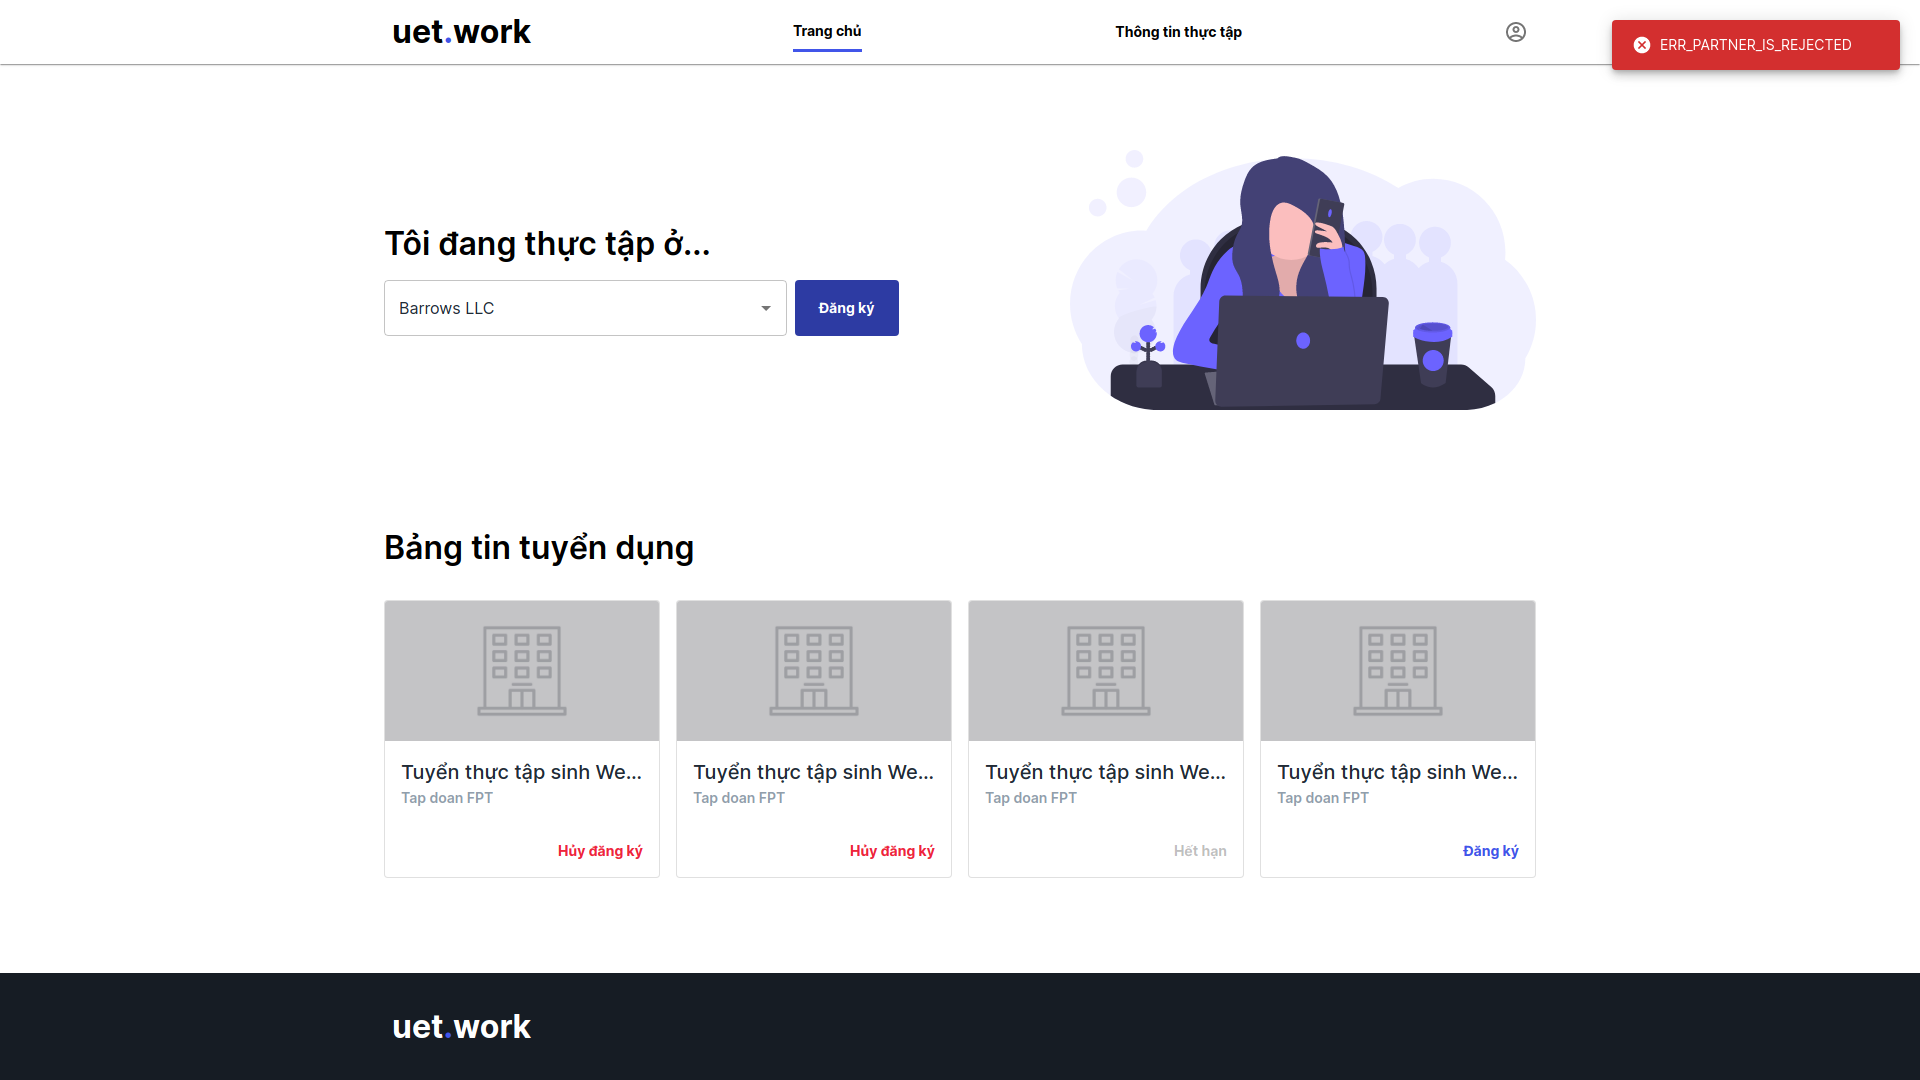
\includegraphics[width=\linewidth]{./images/image40.png}
	\caption{Luồng \emph{Sinh viên đăng ký thực tập}: Đăng ký thất bại}
	\label{fig:student_register_company_failed}
\end{figure}

\paragraph*{Sinh viên xem thông tin thực tập}
Sau khi đăng ký thực tập thành công, sinh viên vào kiểm tra thông tin thực tập của bản thân. Tại đây, sinh viên có thể xem thông tin công ty thực tập đã đúng chưa,  giảng viên hướng dẫn là ai, và nộp báo cáo.

Hình \ref{fig:view_internship_page} mô tả màn hình trang thông tin thực tập.

\begin{figure}[]
	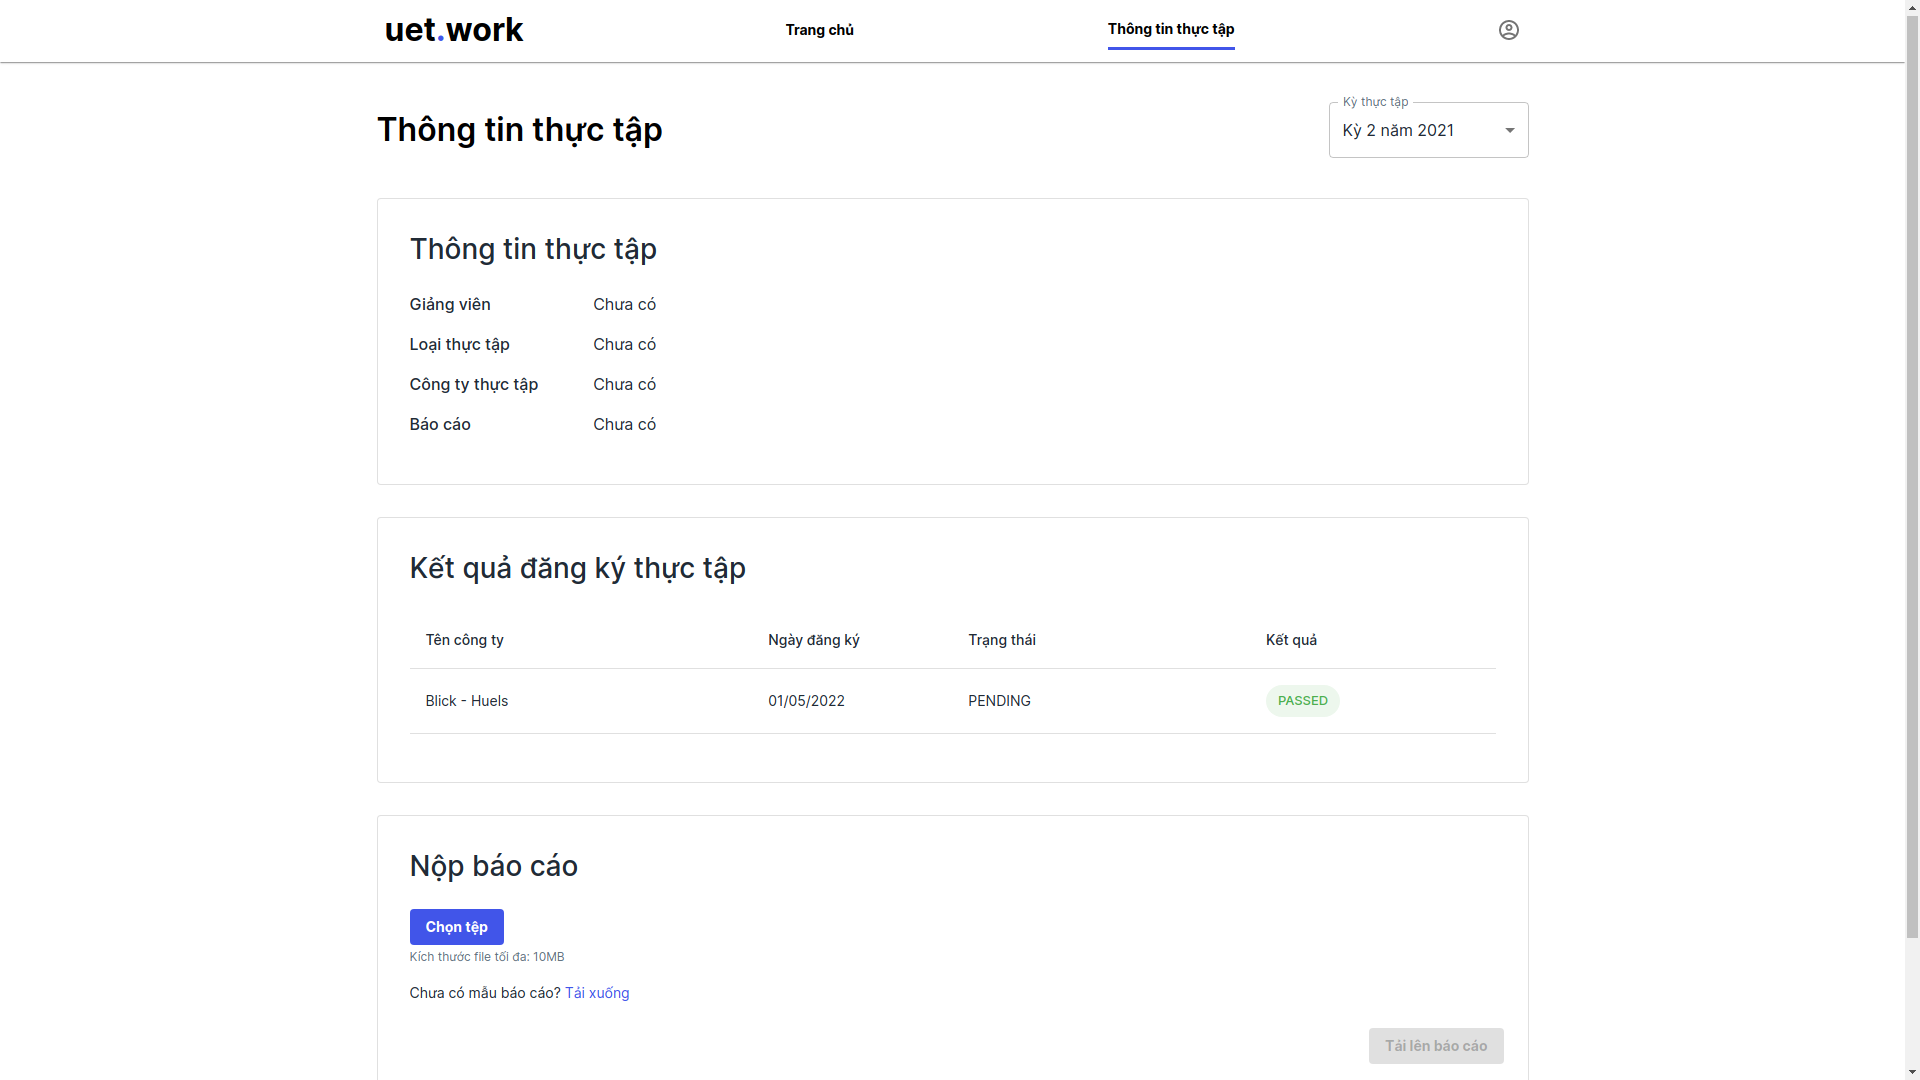
\includegraphics[width=\linewidth]{./images/image17.png}
	\caption{Luồng \emph{Sinh viên xem thông tin thực tập}}
	\label{fig:view_internship_page}
\end{figure}

\paragraph*{Sinh viên nộp báo cáo thực tập}

\begin{itemize}
	\item Hình \ref{fig:student_internship_info}: Sinh viên truy cập trang thông tin thực tập và kéo xuống phần Nộp báo cáo. 
	\item Hình \ref{fig:student_choose_file}: Sinh viên chọn tệp.
	\item Hình \ref{fig:student_upload_report}: Sinh viên tải lên báo cáo.
\end{itemize}

\begin{figure}[]
	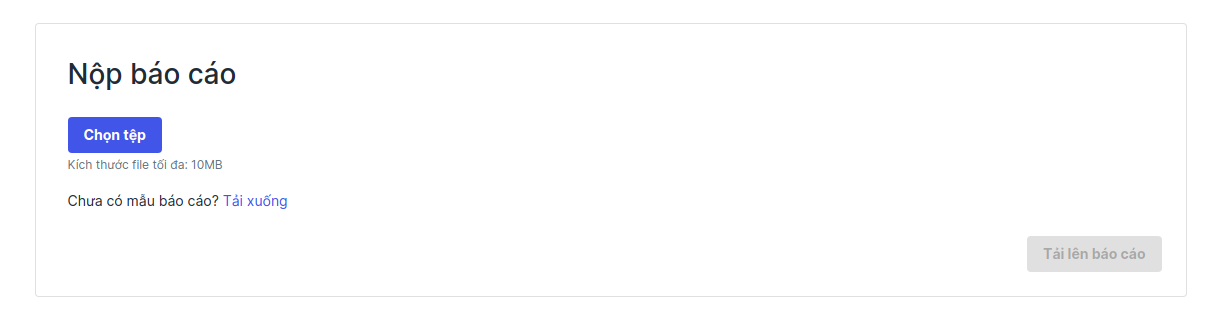
\includegraphics[width=\linewidth]{./images/image41.png}
	\caption{Luồng \emph{Sinh viên nộp báo cáo}: Truy cập phần nộp báo cáo}
	\label{fig:student_internship_info}
\end{figure}

\begin{figure}[]
	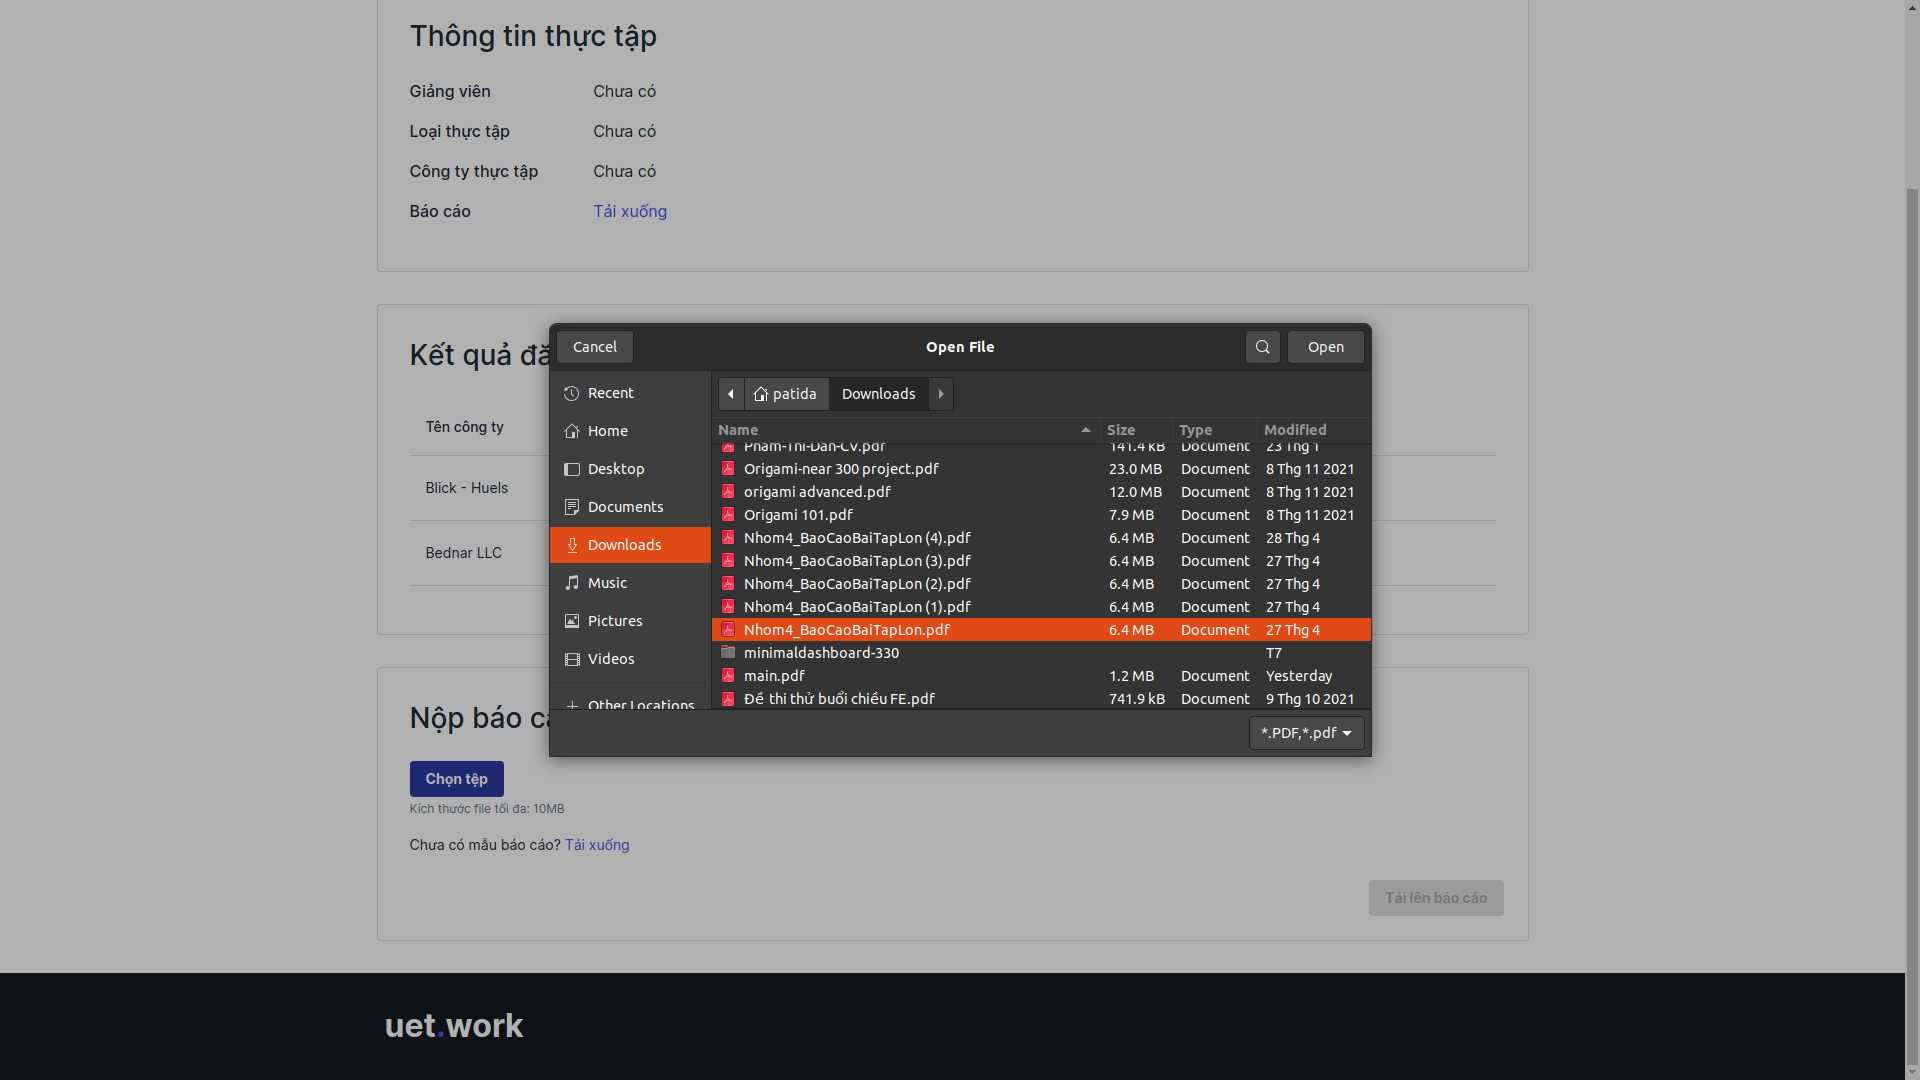
\includegraphics[width=\linewidth]{./images/image42.png}
	\caption{Luồng \emph{Sinh viên nộp báo cáo}: Chọn tệp}
	\label{fig:student_choose_file}
\end{figure}

\begin{figure}[]
	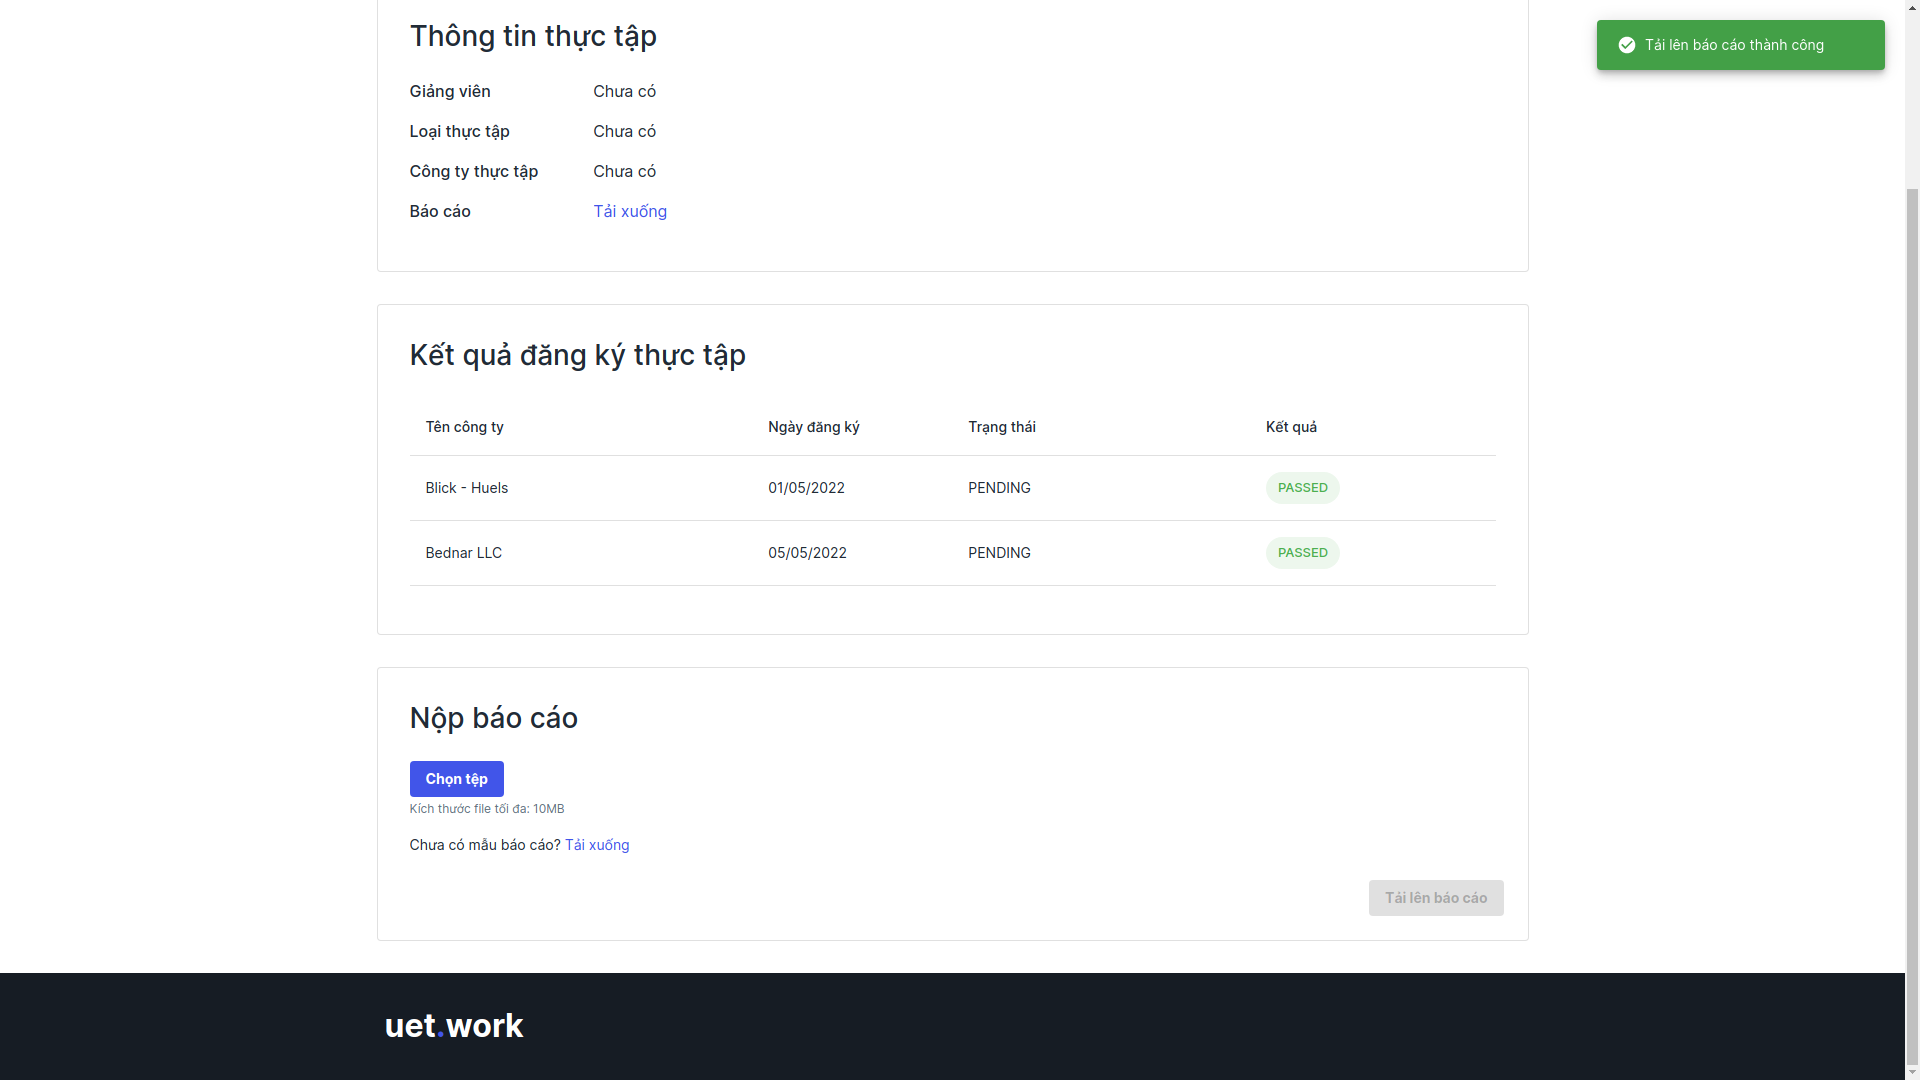
\includegraphics[width=\linewidth]{./images/image43.png}
	\caption{Luồng \emph{Sinh viên nộp báo cáo}: Tải lên báo cáo}
	\label{fig:student_upload_report}
\end{figure}

\paragraph*{Sinh viên xem thông tin cá nhân}
Sinh viên truy cập trang thông tin cá nhân. Tại đây sinh viên có thể sửa thông tin cá nhân, đổi mật khẩu.

Hình \ref{fig:view_info_page} mô tả màn hình trang thông tin cá nhân.

\begin{figure}[]
	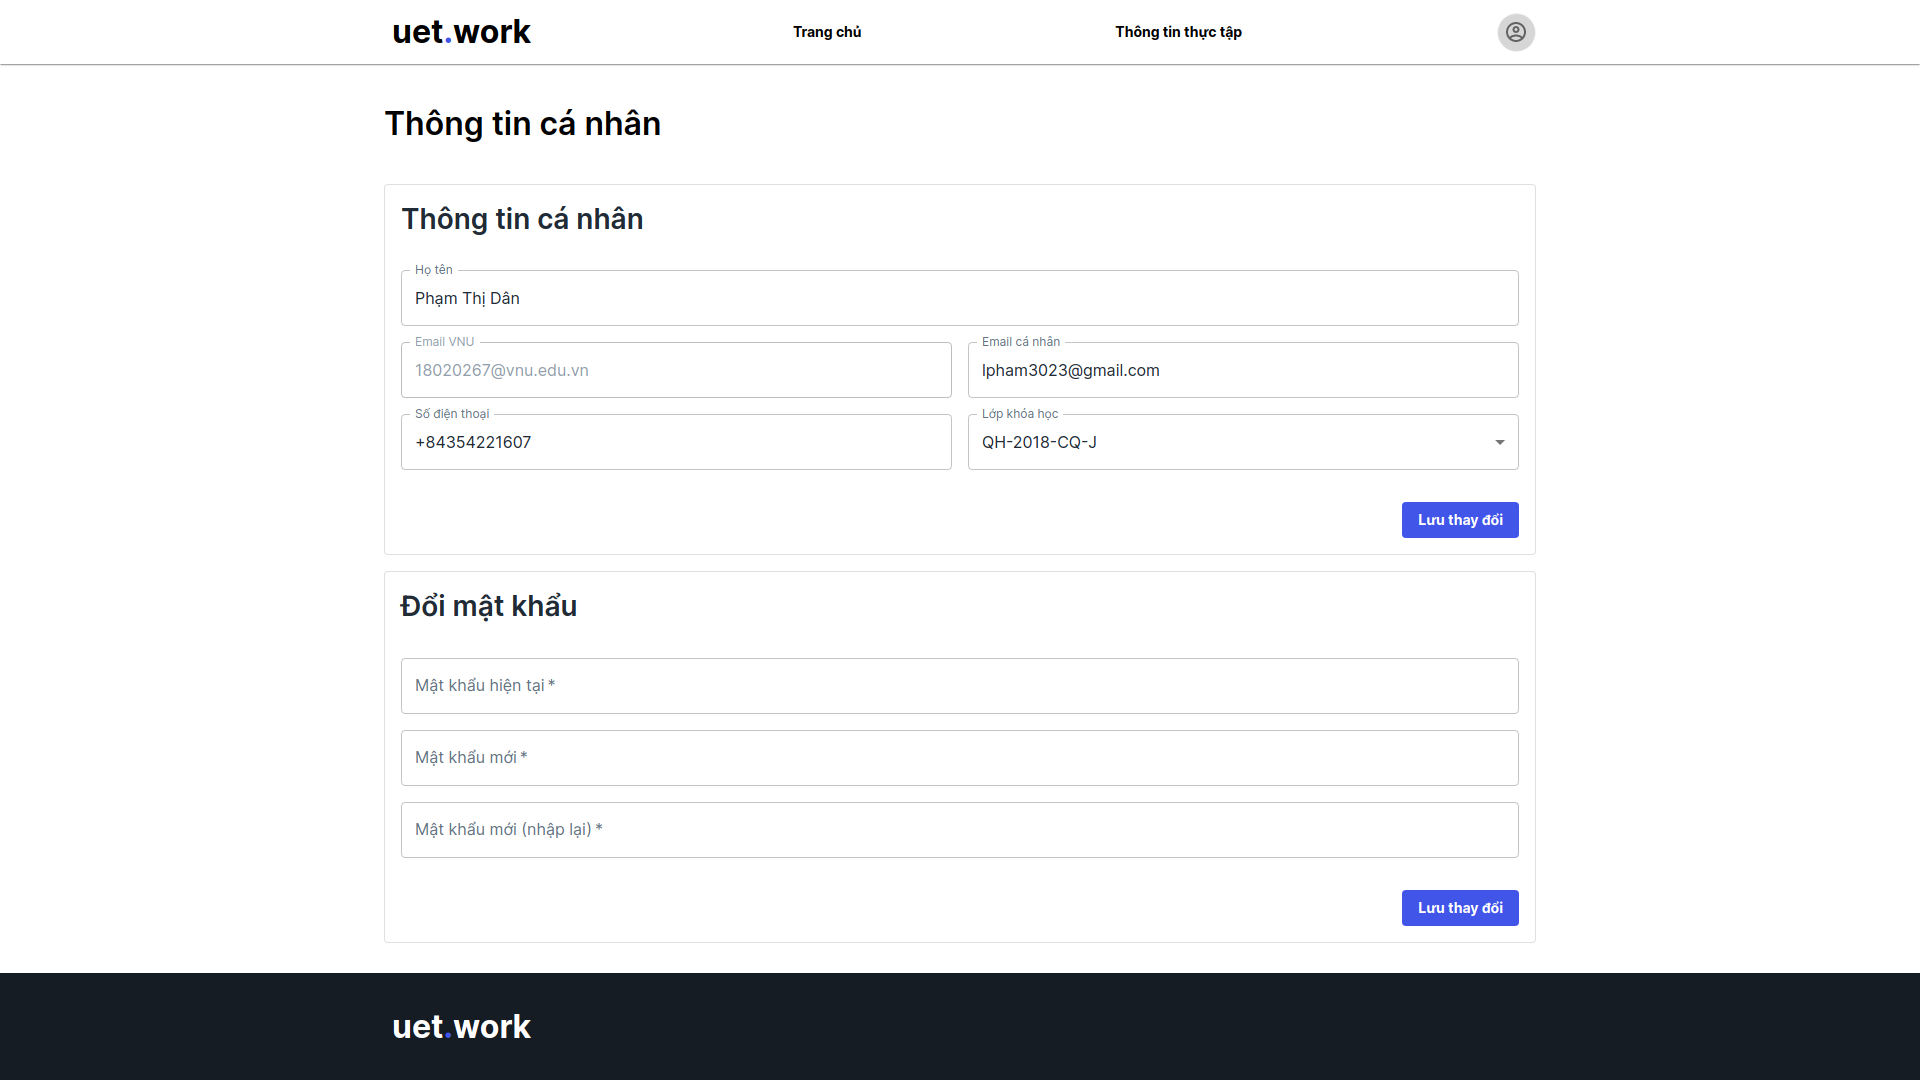
\includegraphics[width=\linewidth]{./images/image44.png}
	\caption{Luồng \emph{Sinh viên xem thông tin cá nhân}}
	\label{fig:view_info_page}
\end{figure}

\paragraph*{Sinh viên thay đổi thông tin cá nhân}

\begin{itemize}
	\item Hình \ref{fig:student_access_info}: Sinh viên truy cập phần thông tin cá nhân. 
	\item Hình \ref{fig:student_edit_info}: Sinh viên sửa thông tin cá nhân, đổi mật khẩu.
\end{itemize}

\begin{figure}[]
	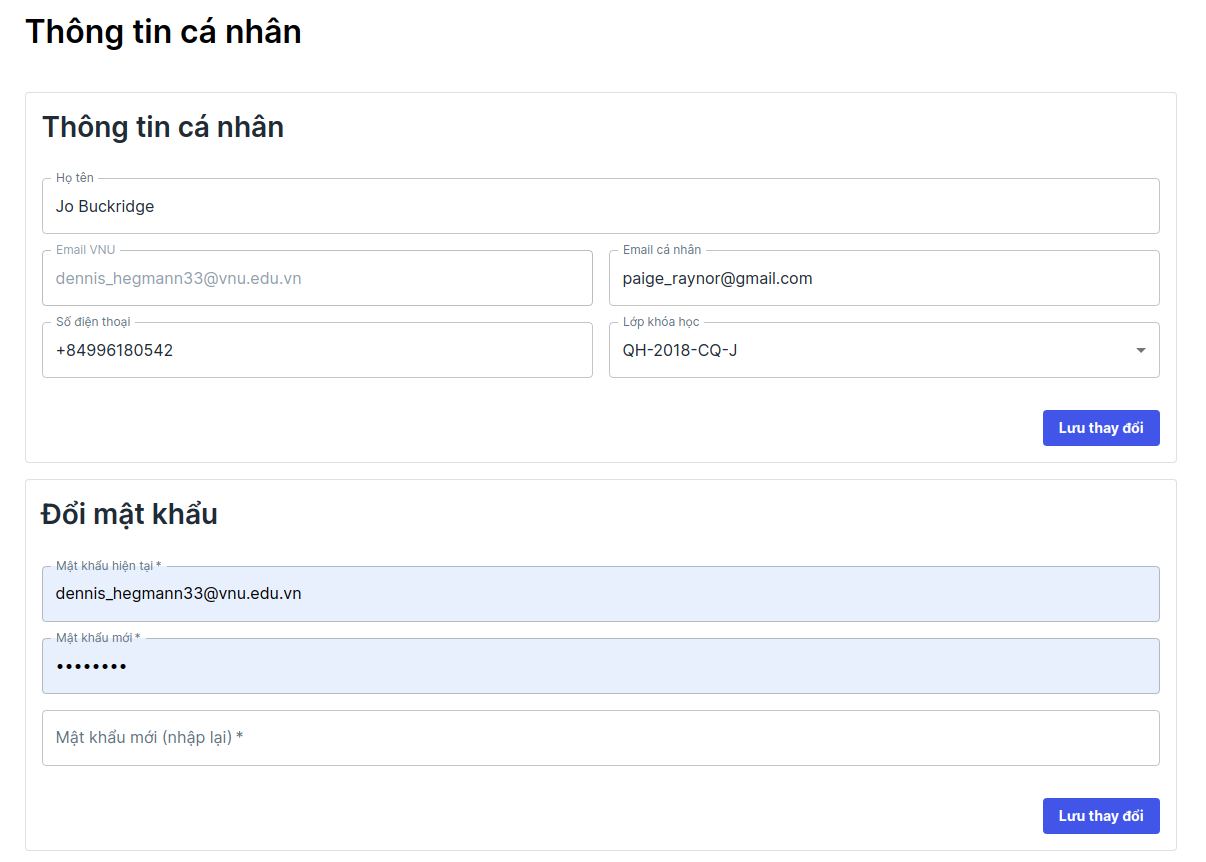
\includegraphics[width=\linewidth]{./images/image45.png}
	\caption{Luồng \emph{Sinh viên thay đổi thông tin cá nhân}: Truy cập trang thông tin cá nhân}
	\label{fig:student_access_info}
\end{figure}

\begin{figure}[]
	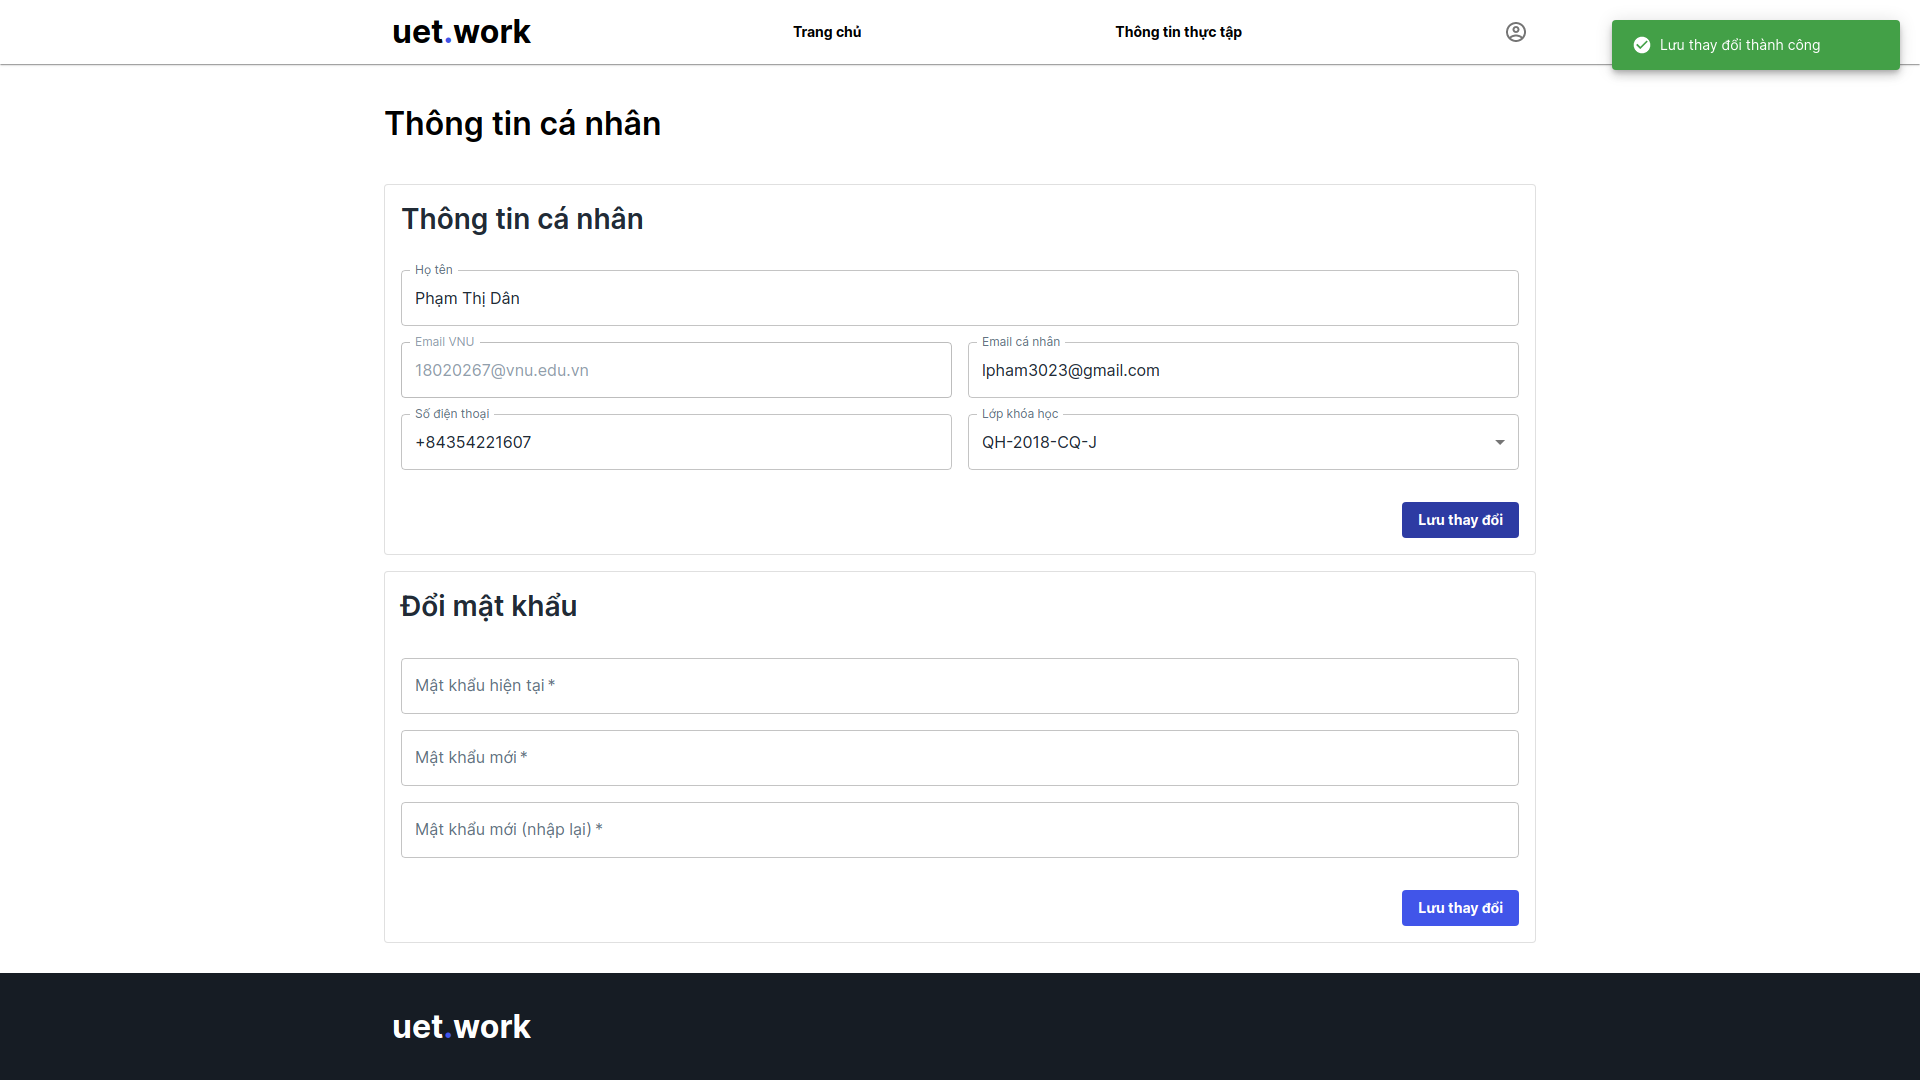
\includegraphics[width=\linewidth]{./images/image46.png}
	\caption{Luồng \emph{Sinh viên thay đổi thông tin cá nhân}: Sinh viên thay đổi thông tin cá nhân}
	\label{fig:student_edit_info}
\end{figure}

\subsection{Luồng sử dụng của giảng viên}

\paragraph*{Đọc báo cáo và chấm điểm cho sinh viên}

Tại đây, giảng viên tải xuống file báo cáo của sinh viên. Sau khi đọc và cho điểm xong, giảng viên thực hiện \emph{Thêm điểm} cho sinh viên.

Hình \ref{fig:working_student_page} mô tả màn hình danh sách sinh viên đang hướng dẫn.

\begin{figure}[]
	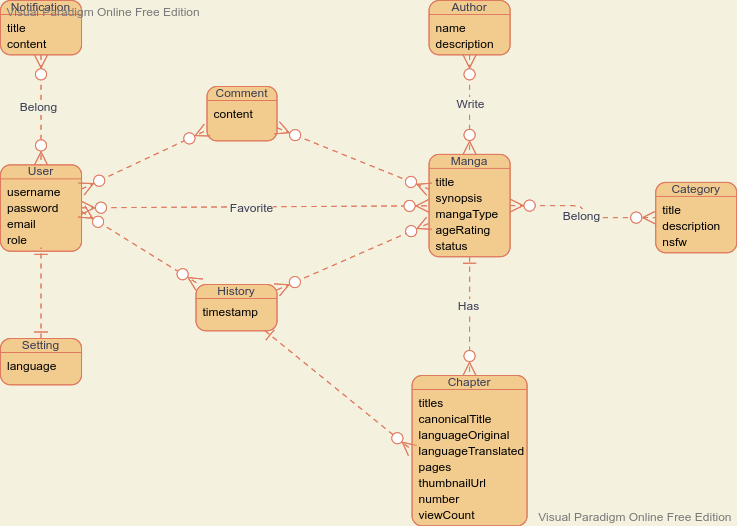
\includegraphics[width=\linewidth]{./images/image8.png}
	\caption{Màn hình danh sách sinh viên đang hướng dẫn}
	\label{fig:working_student_page}
\end{figure}

\subsection{Luồng sử dụng của đối tác}

\paragraph*{Thêm bài đăng tuyển dụng}

Tại trang Thêm bài đăng, đối tác thêm tiêu đề, nội dung chi tiết, số lượng tuyển dụng, ngày bắt đầu, ngày kết thúc, người liên hệ để tạo một bài đăng mới.

Hình \ref{fig:add_post_page} mô tả màn hình thêm bài đăng của đối tác.

\paragraph*{Chấp nhận / Từ chối yêu cầu thực tập}

Sau khi có các sinh viên đăng ký thực tập tại công ty, đối tác có thể vào trang Yêu cầu đăng ký thực tập để chấp nhận hoặc từ chối yêu cầu của sinh viên.

Hình \ref{fig:approve_or_reject_request} mô tả màn hình chấp nhận / từ chối yêu cầu thực tập.

\begin{figure}[]
	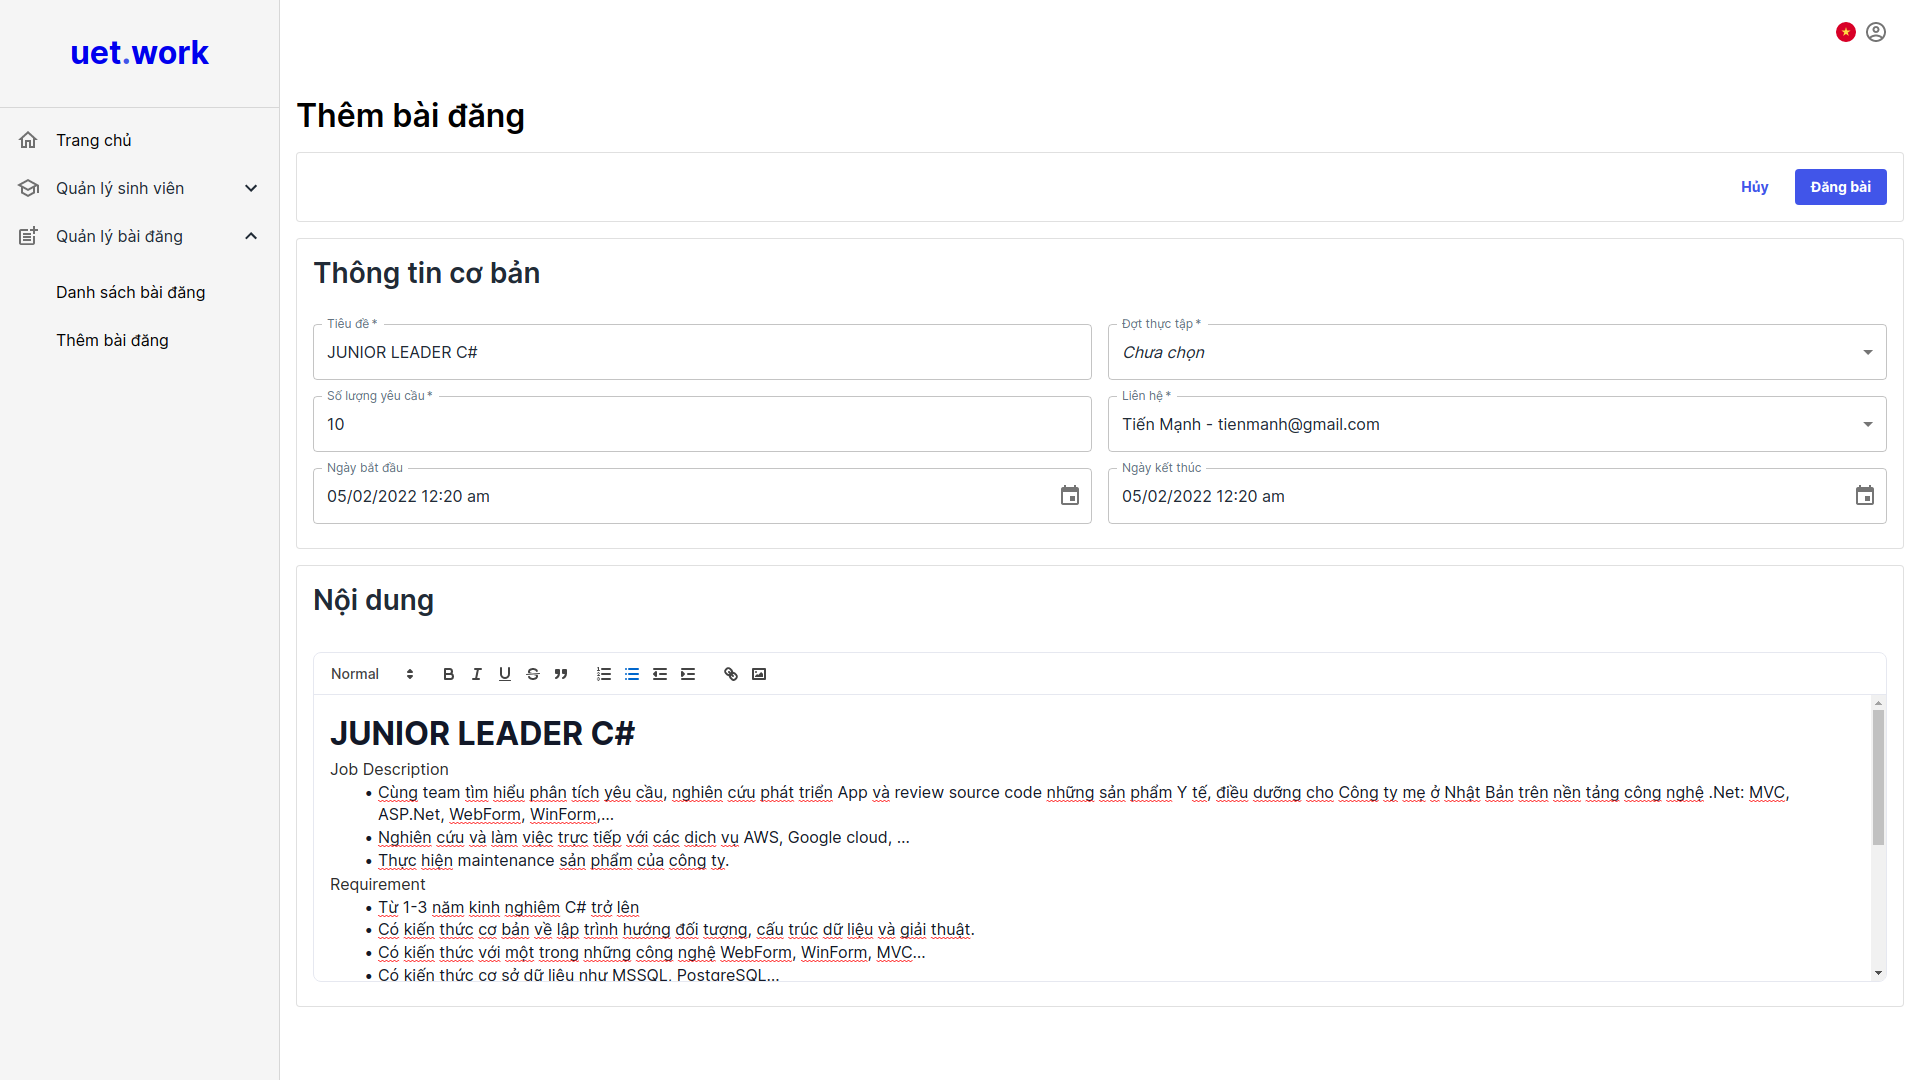
\includegraphics[width=\linewidth]{./images/image18.png}
	\caption{Màn hình thêm bài đăng mới}
	\label{fig:add_post_page}
\end{figure}

\begin{figure}[]
	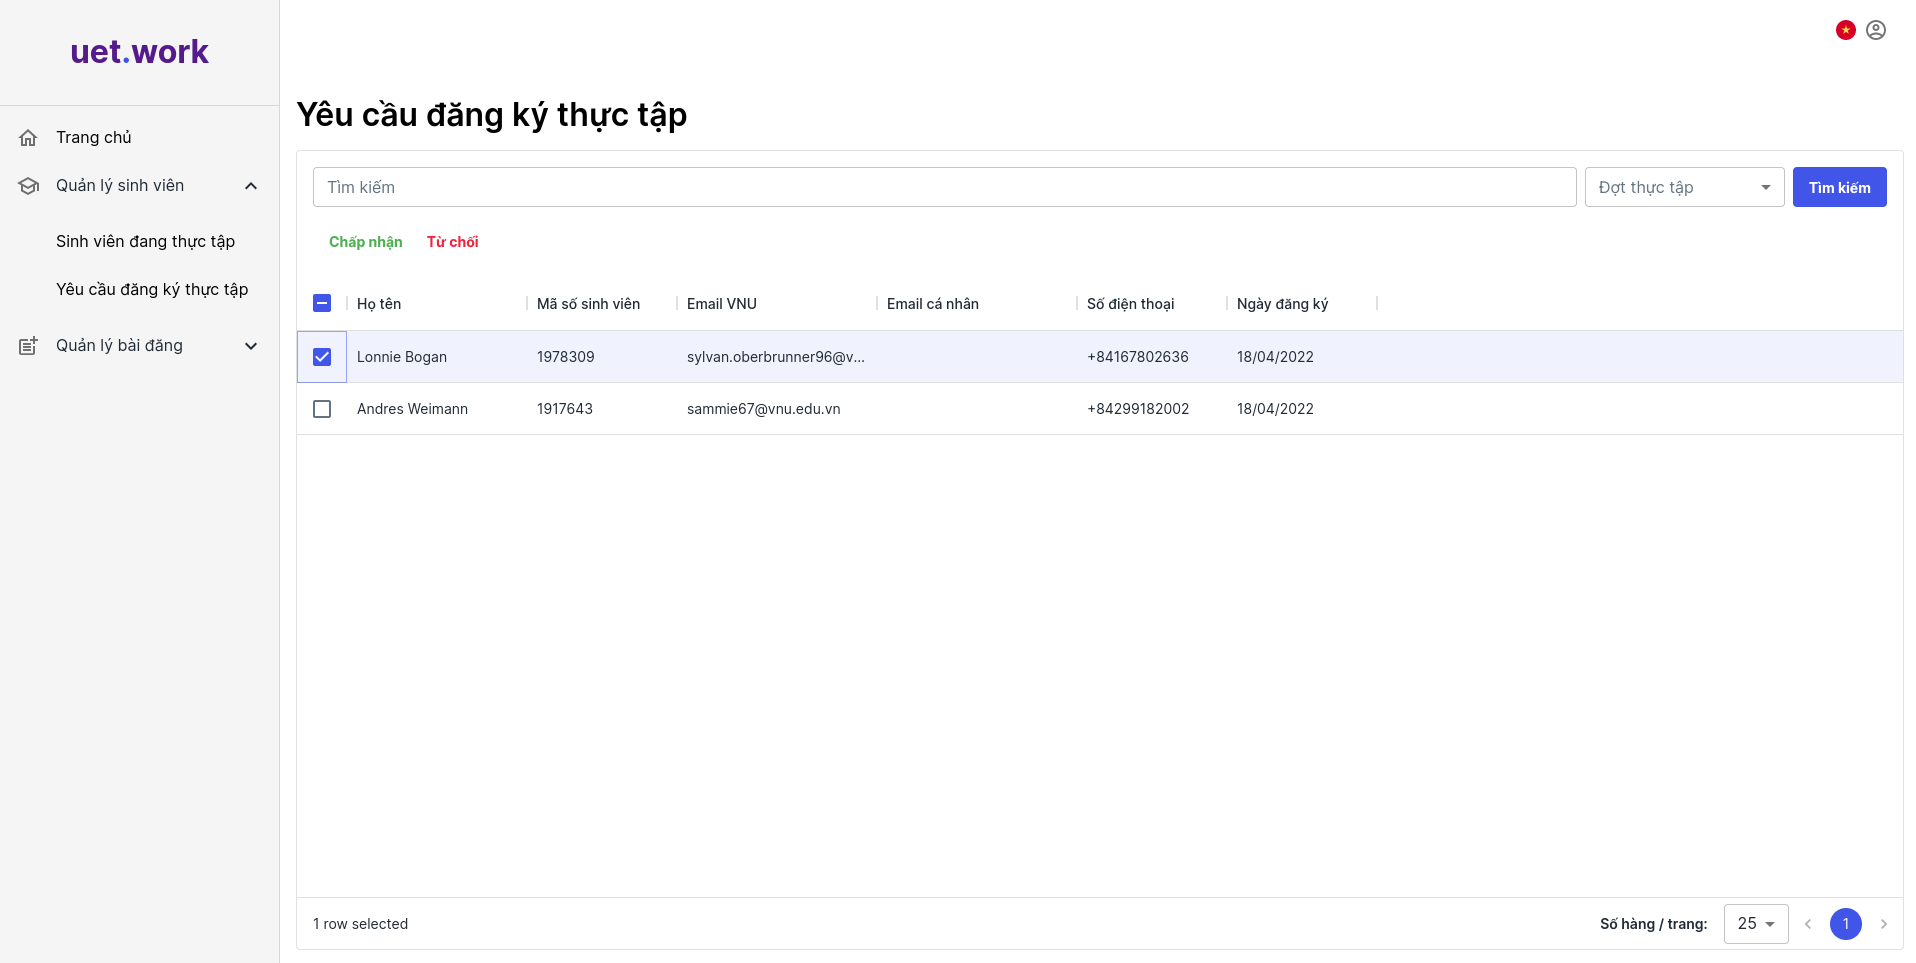
\includegraphics[width=\linewidth]{./images/image29.png}
	\caption{Màn hình chấp nhận / từ chối yêu cầu thực tập }
	\label{fig:approve_or_reject_request}
\end{figure}

\subsection{Luồng sử dụng của quản trị viên Khoa}

\paragraph*{Tạo kỳ thực tập mới}

Quản trị viên Khoa tạo một kỳ thực tập mới, các thông tin bao gồm năm, kỳ, ngày bắt đầu, ngày kết thúc, ngày bắt đầu đăng ký, ngày kết thúc đăng ký.

Hình \ref{fig:add_term_page} mô tả màn hình tạo kỳ thực tập mới.

\paragraph*{Tạo kỳ thực tập thành công}

Sau khi tạo thành công, hệ thống phản hồi lại thông báo và cập nhật danh sách các kỳ thực tập.

Hình \ref{fig:add_term_success} mô tả màn hình tạo kỳ thực tập mới thành công.

\paragraph*{Gán giảng viên cho sinh viên}

Sau khi sinh viên đã chốt nơi thực tập, quản trị viên chọn các sinh viên rồi thực hiện gán giảng viên.

Hình \ref{fig:assign_lecturer} mô tả màn hình gán giảng viên cho sinh viên.

\paragraph*{Chấp nhận / Từ chối công ty}

Quản trị viên chọn một công ty đang ở chế độ Pending và thực hiện chấp nhận hay từ chối công ty.

Hình \ref{fig:reject_or_approve_company} mô tả màn hình Chấp nhận / Từ chối công ty.

\begin{figure}[]
	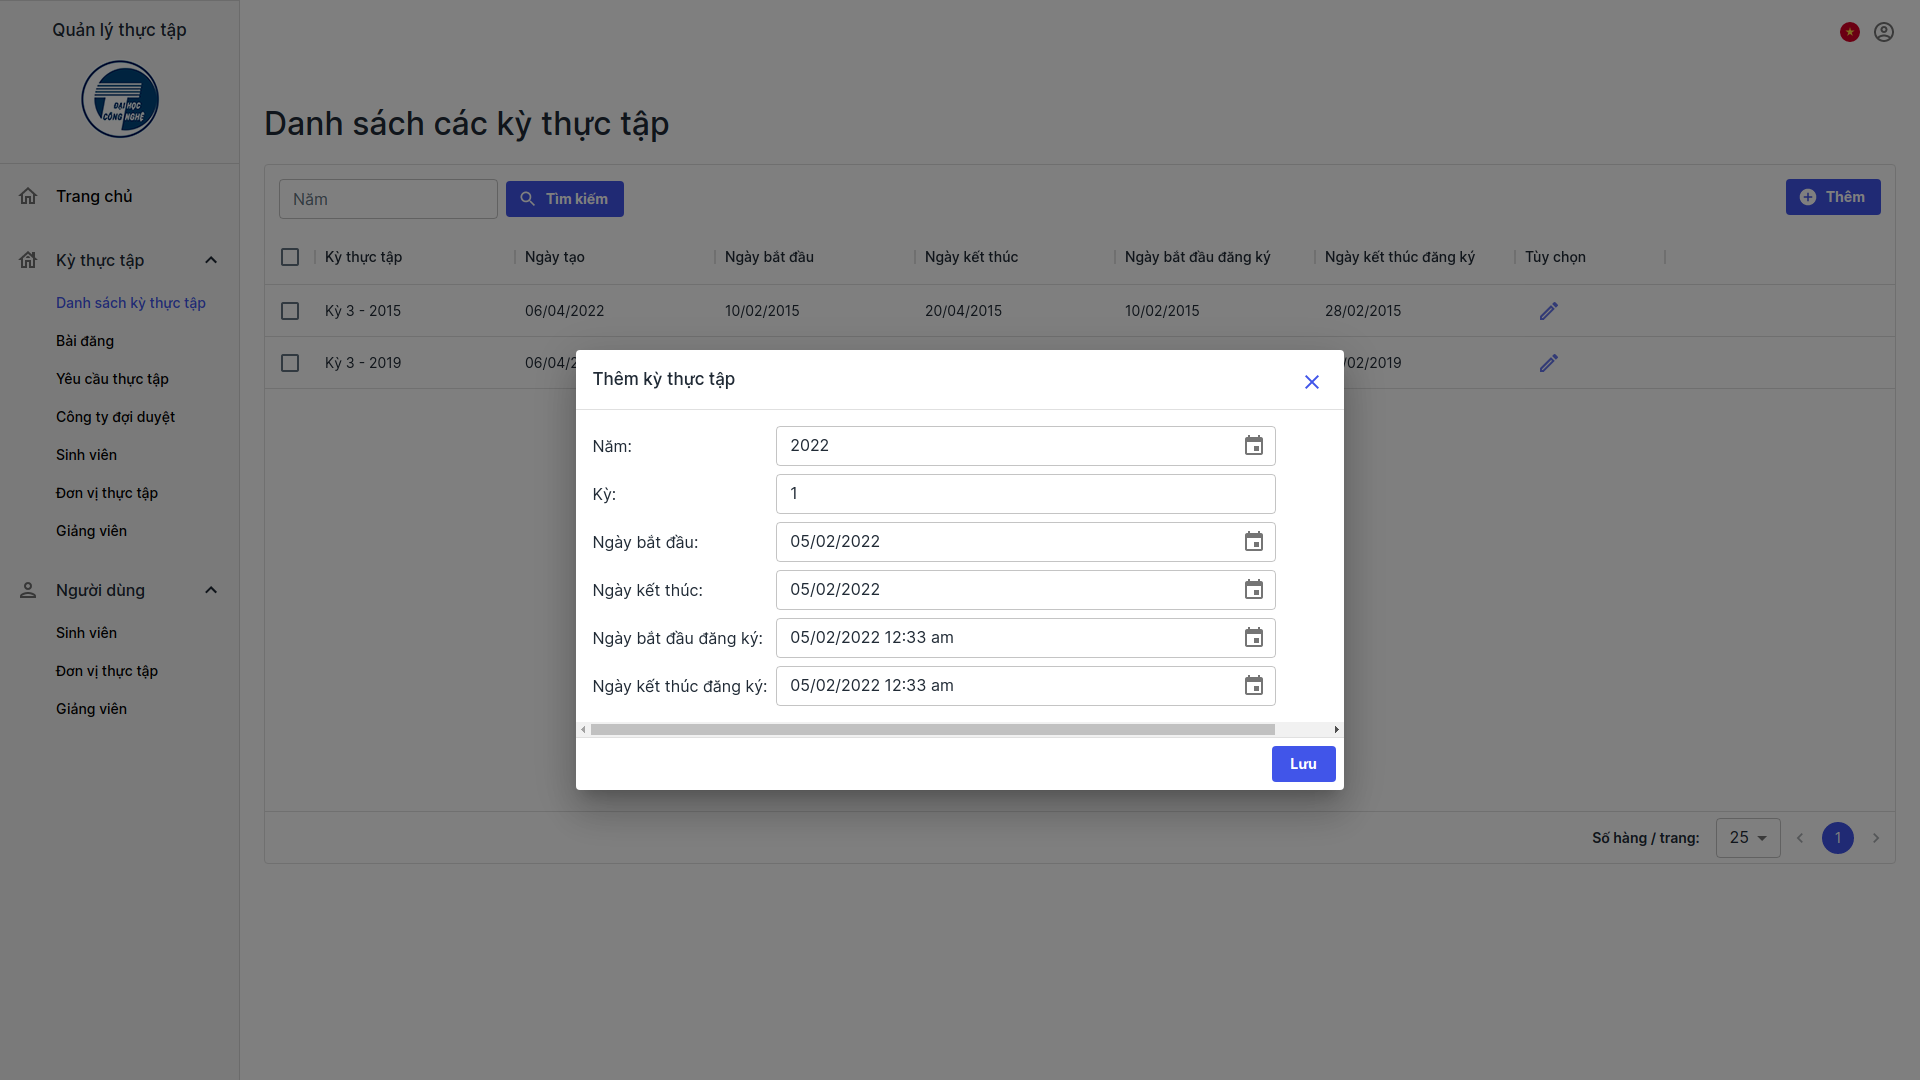
\includegraphics[width=\linewidth]{./images/image19.png}
	\caption{Màn hình tạo kỳ thực tập mới}
	\label{fig:add_term_page}
\end{figure}

\begin{figure}[]
	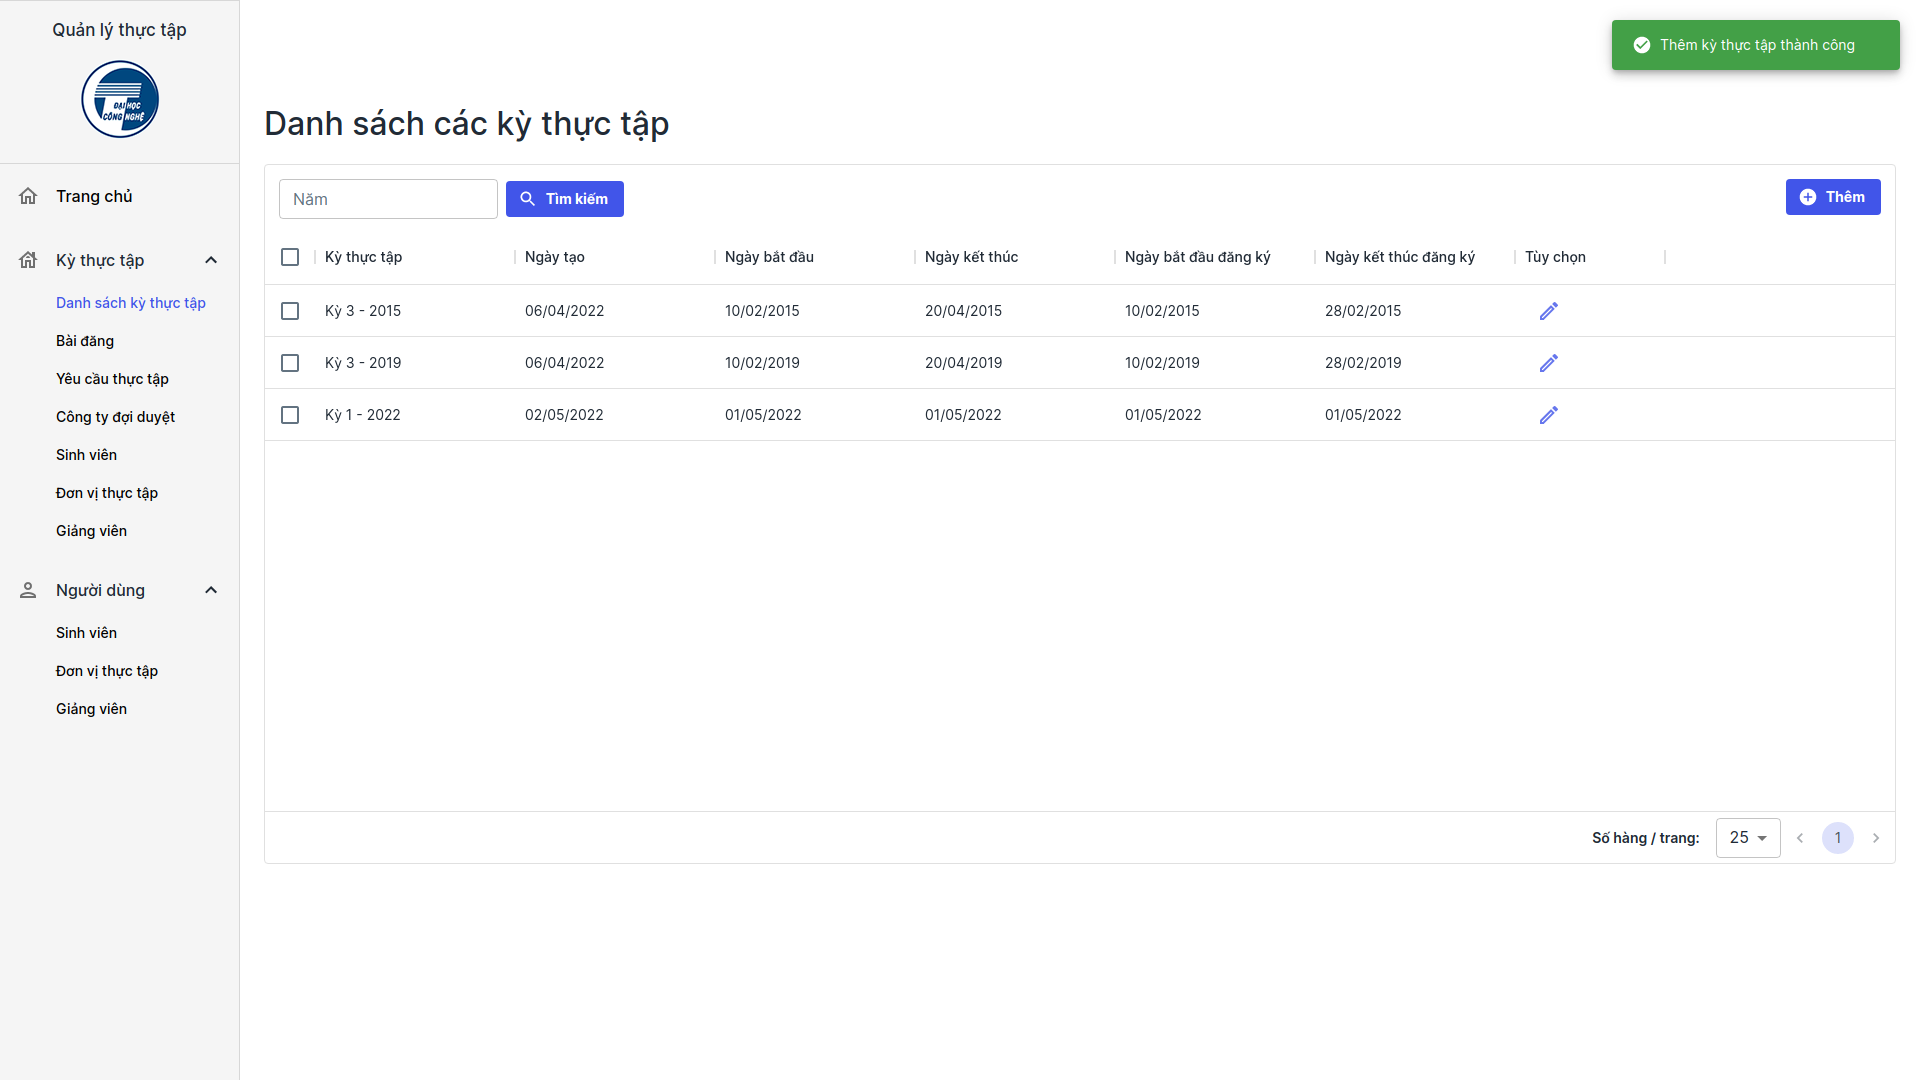
\includegraphics[width=\linewidth]{./images/image20.png}
	\caption{Màn hình tạo kỳ thực tập mới thành công}
	\label{fig:add_term_success}
\end{figure}

\begin{figure}[]
	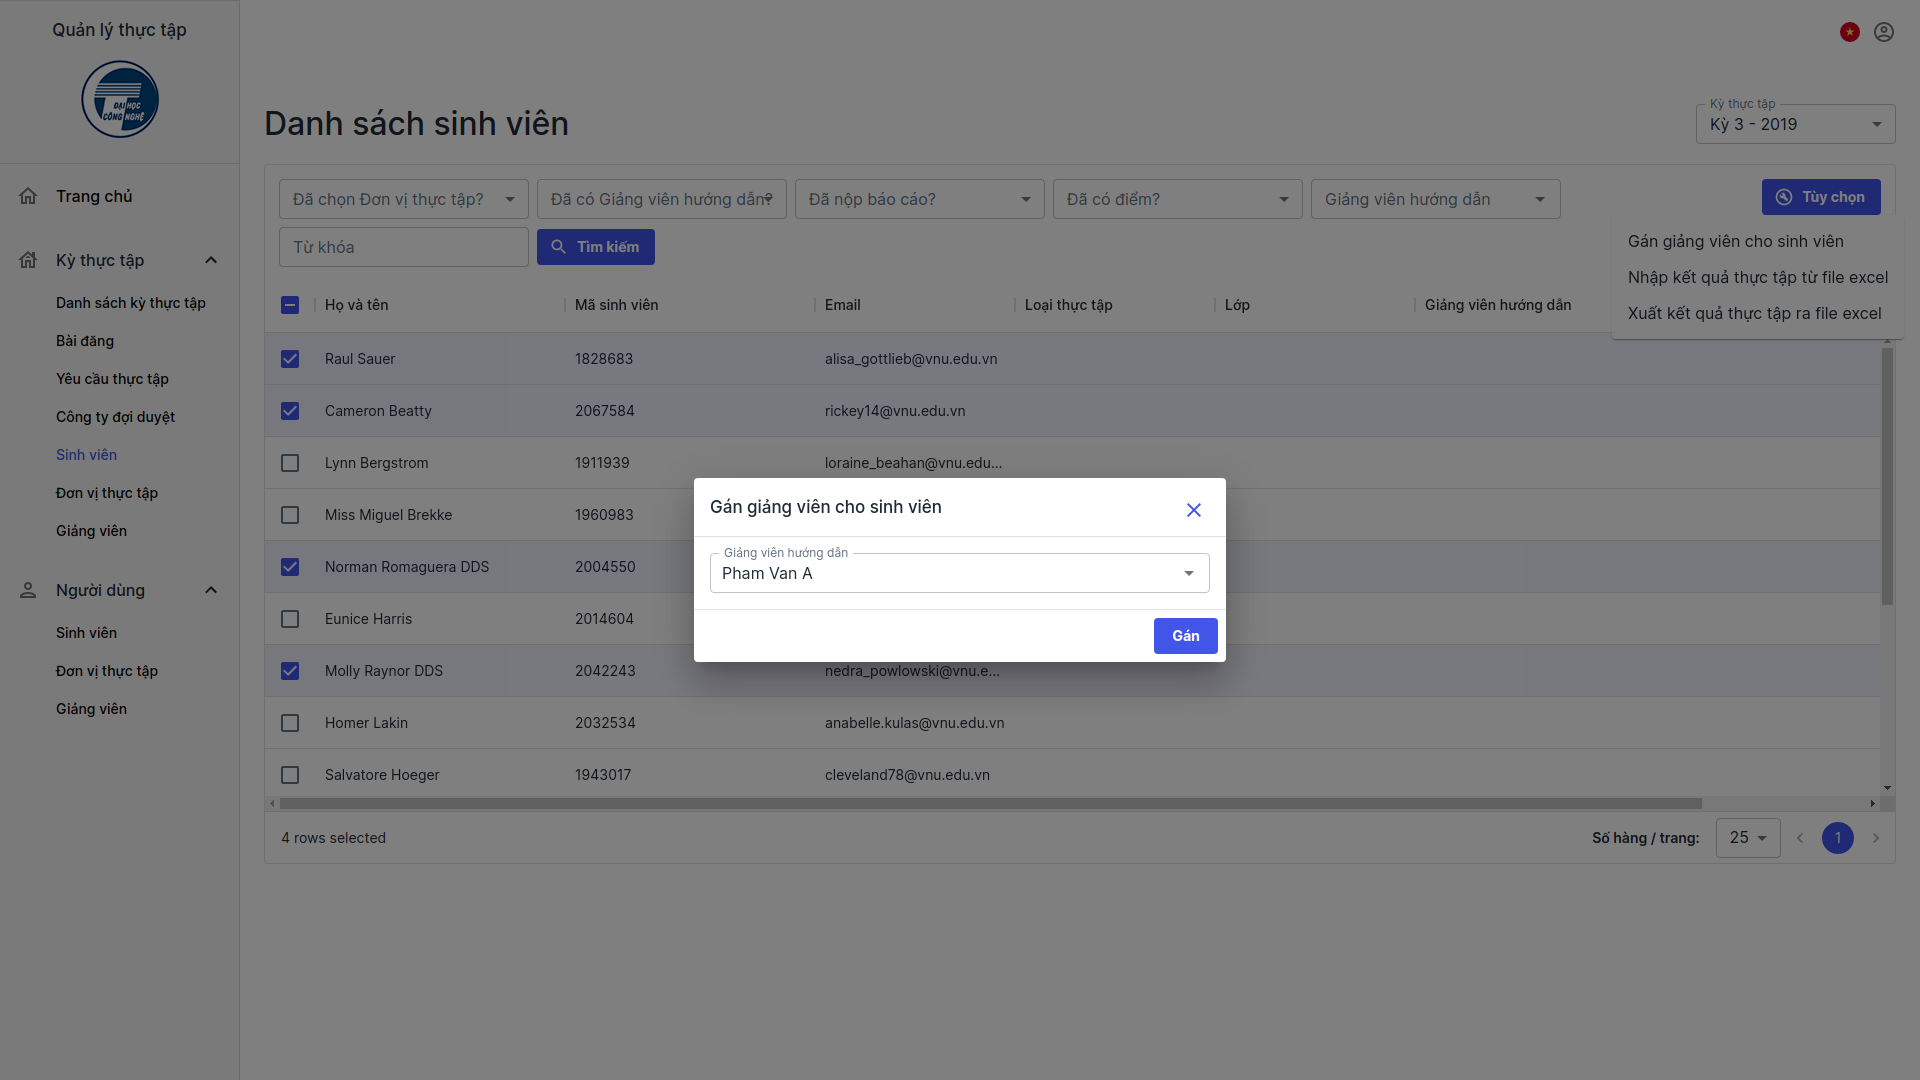
\includegraphics[width=\linewidth]{./images/image22.png}
	\caption{Màn hình gán giảng viên cho sinh viên}
	\label{fig:assign_lecturer}
\end{figure}

\begin{figure}[]
	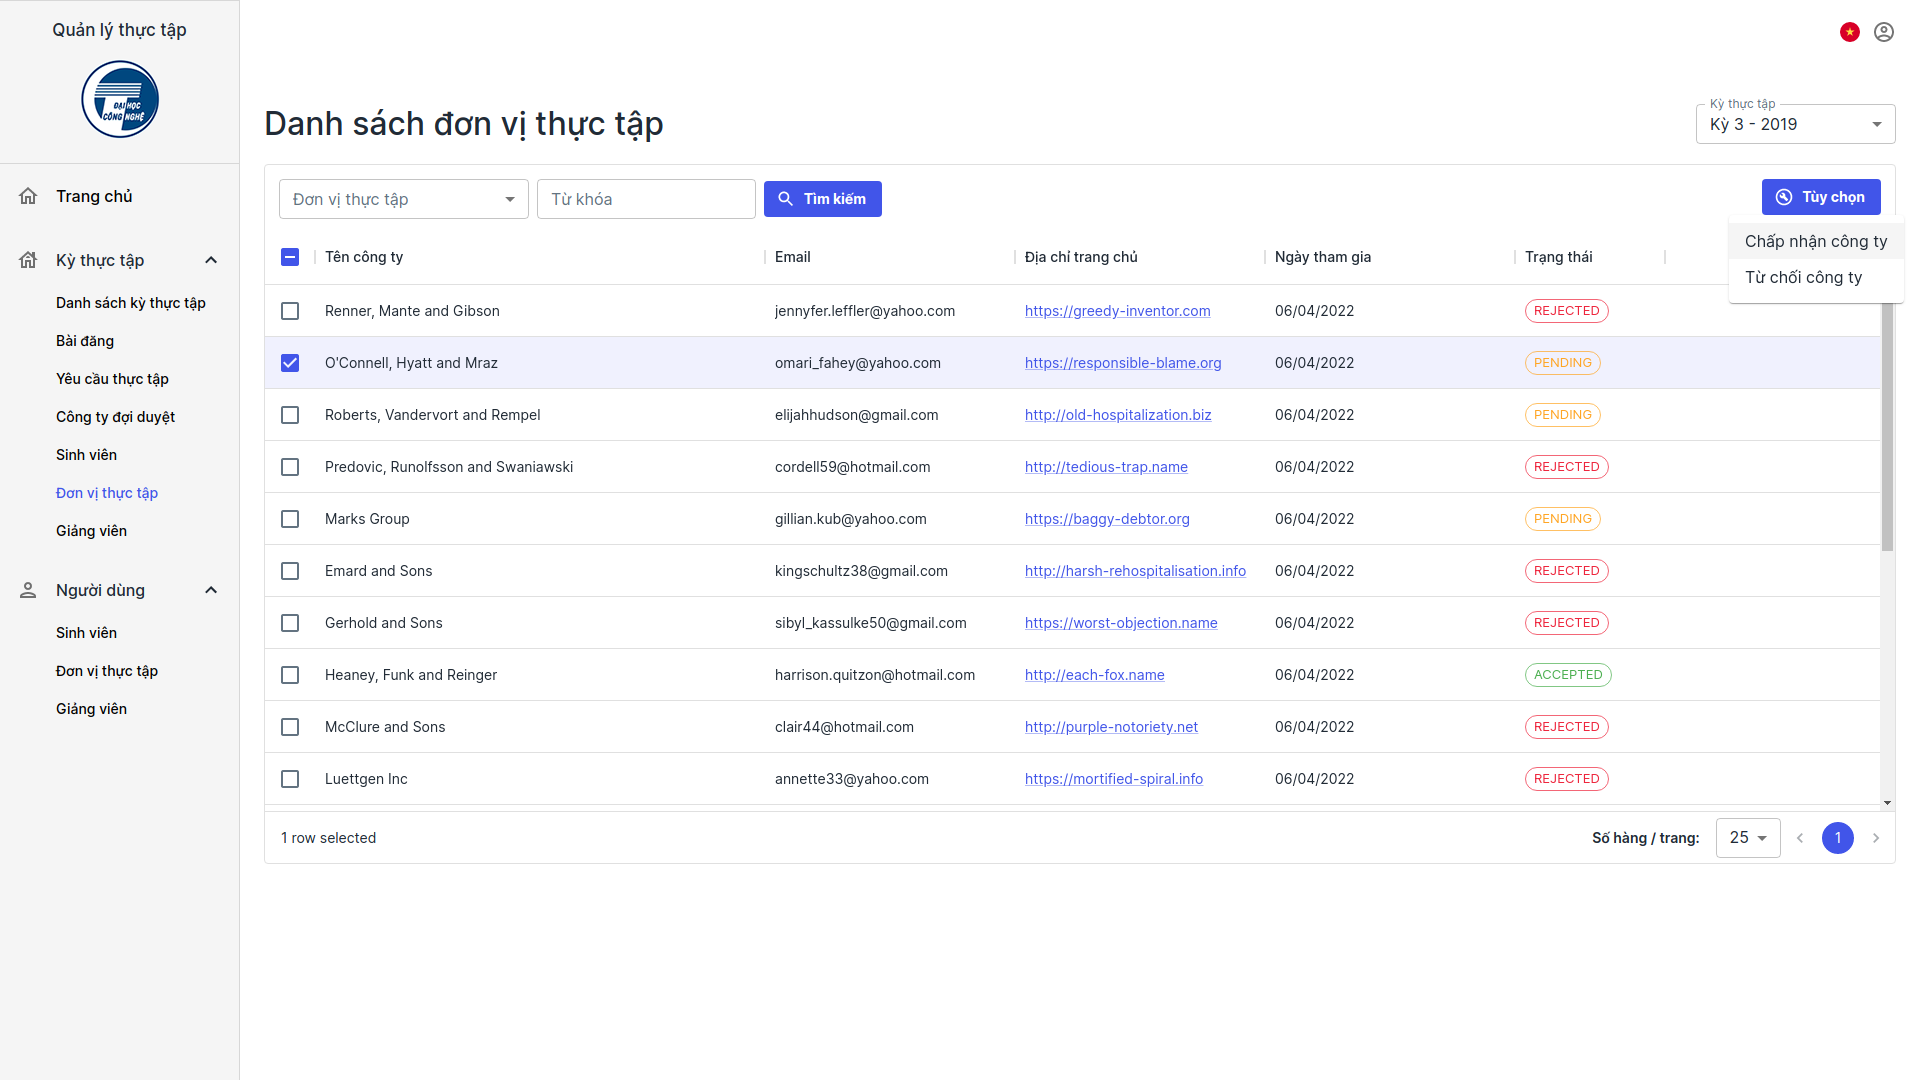
\includegraphics[width=\linewidth]{./images/image21.png}
	\caption{Màn hình Chấp nhận / Từ chối công ty}
	\label{fig:reject_or_approve_company}
\end{figure}

\subsection{Luồng sử dụng của quản trị viên hệ thống}

\paragraph*{Tạo Khoa mới}

Quản trị viên thực hiện tạo Khoa mới gồm có: tên khoa, email quản trị viên Khoa.

Hình \ref{fig:add_org} mô tả màn hình tạo Khoa mới.

\paragraph*{Tạo Khoa mới thành công}

Sau khi tạo thành công, một email được gửi đến hòm thư cung cấp mật khẩu cho quản trị viên Khoa.

% Hình \ref{fig:add_org_success} mô tả màn hình hòm thư sau khi tạo Khoa mới thành công.

\paragraph*{Tạo Lớp mới}

Quản trị viên thực hiện tạo lớp mới gồm các thông tin: tên lớp, chương trình giảng dạy.

Hình \ref{fig:add_class} mô tả màn hình tạo Lớp mới.

\paragraph*{Nhập vào Danh sách sinh viên}

Từ màn hình Sinh viên, quản trị viên chọn chức năng Nhập danh sách từ file excel để tải lên danh sách sinh viên của hệ thống.

Hình \ref{fig:choose_file} mô tả màn hình chọn file Danh sách sinh viên.

Sau khi chọn xong tệp, dữ liệu ở trong file được hiển thị lại trên màn hình. Quản trị viên chọn chức năng Tải lên để tải lên danh sách sinh viên.

Hình \ref{fig:upload_list} mô tả màn hình tải lên file Danh sách sinh viên.

\begin{figure}[]
	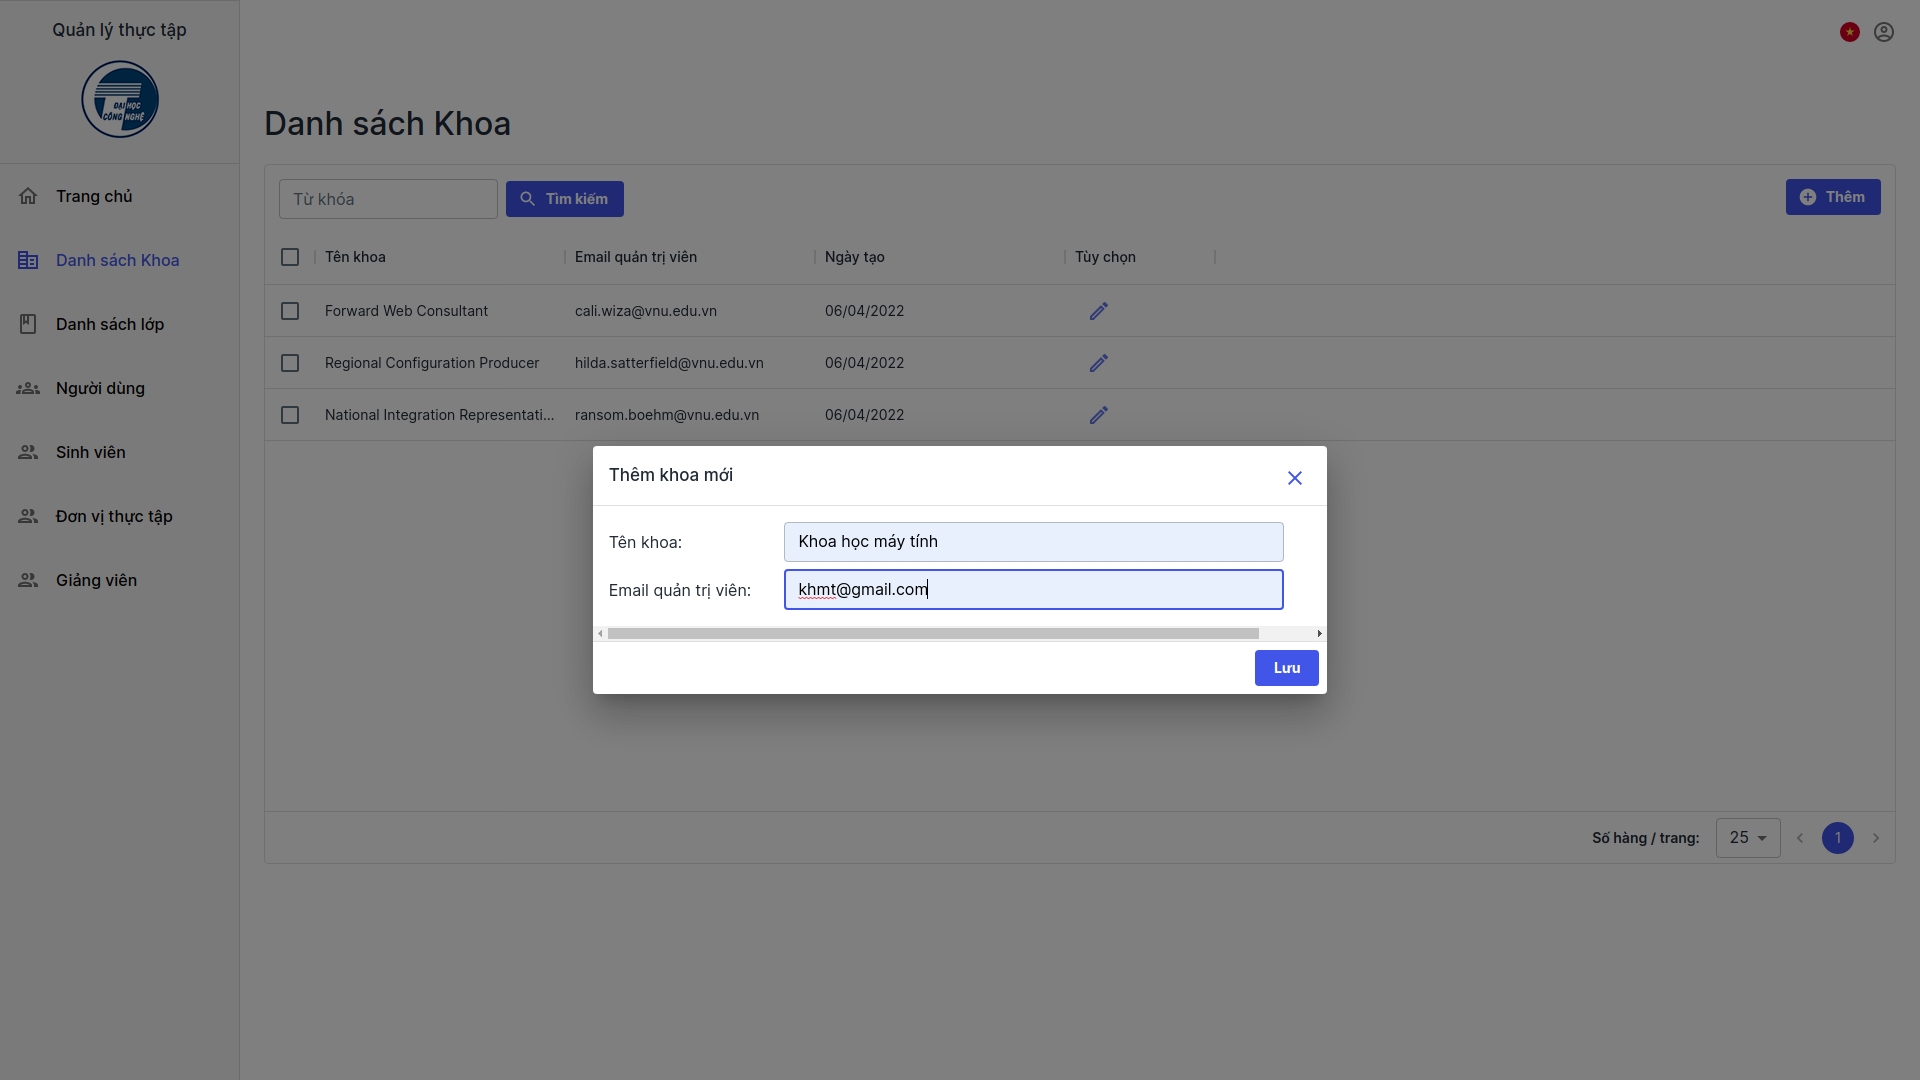
\includegraphics[width=\linewidth]{./images/image23.png}
	\caption{Màn hình tạo Khoa mới}
	\label{fig:add_org}
\end{figure}

% \begin{figure}[]
% 	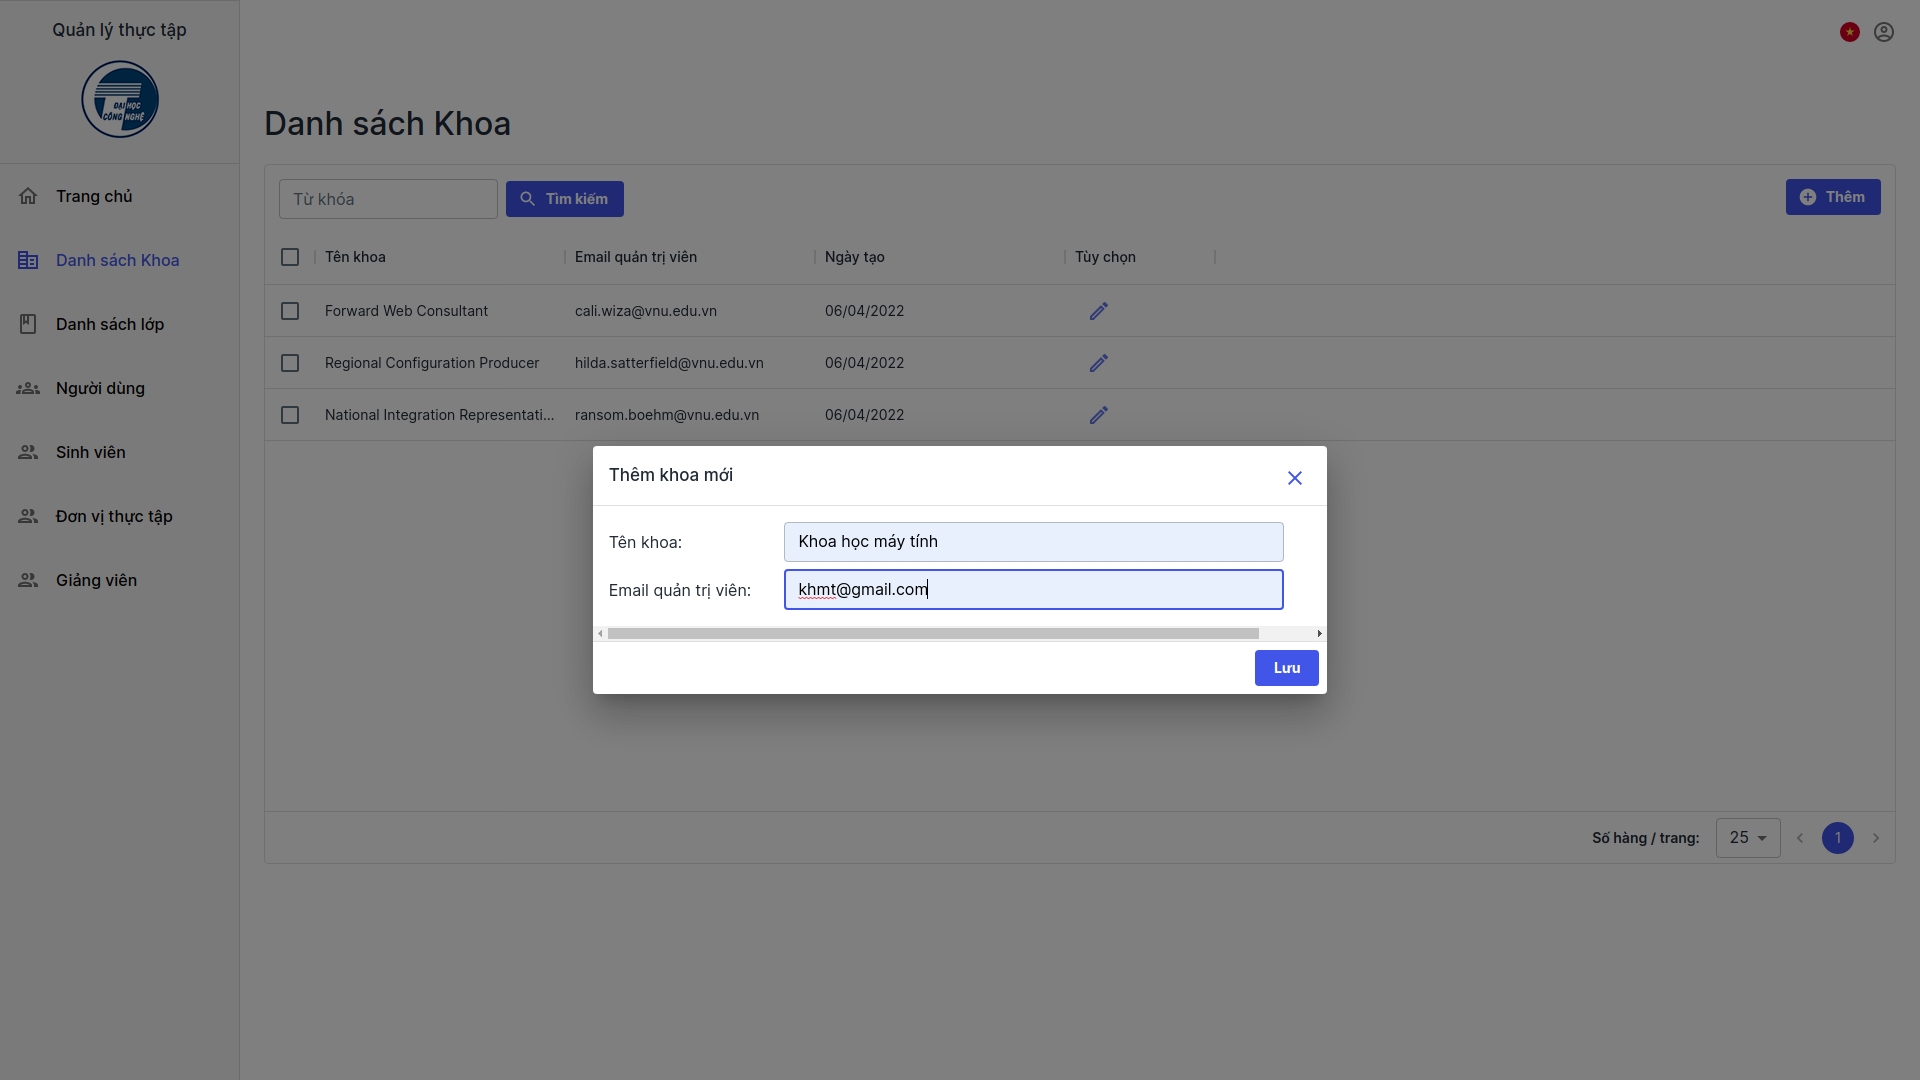
\includegraphics[width=\linewidth]{./images/image23.png} %TODO: replace image
% 	\caption{Màn hình hòm thư sau khi tạo Khoa mới thành côngg}
% 	\label{fig:add_org_success}
% \end{figure}

\begin{figure}[]
	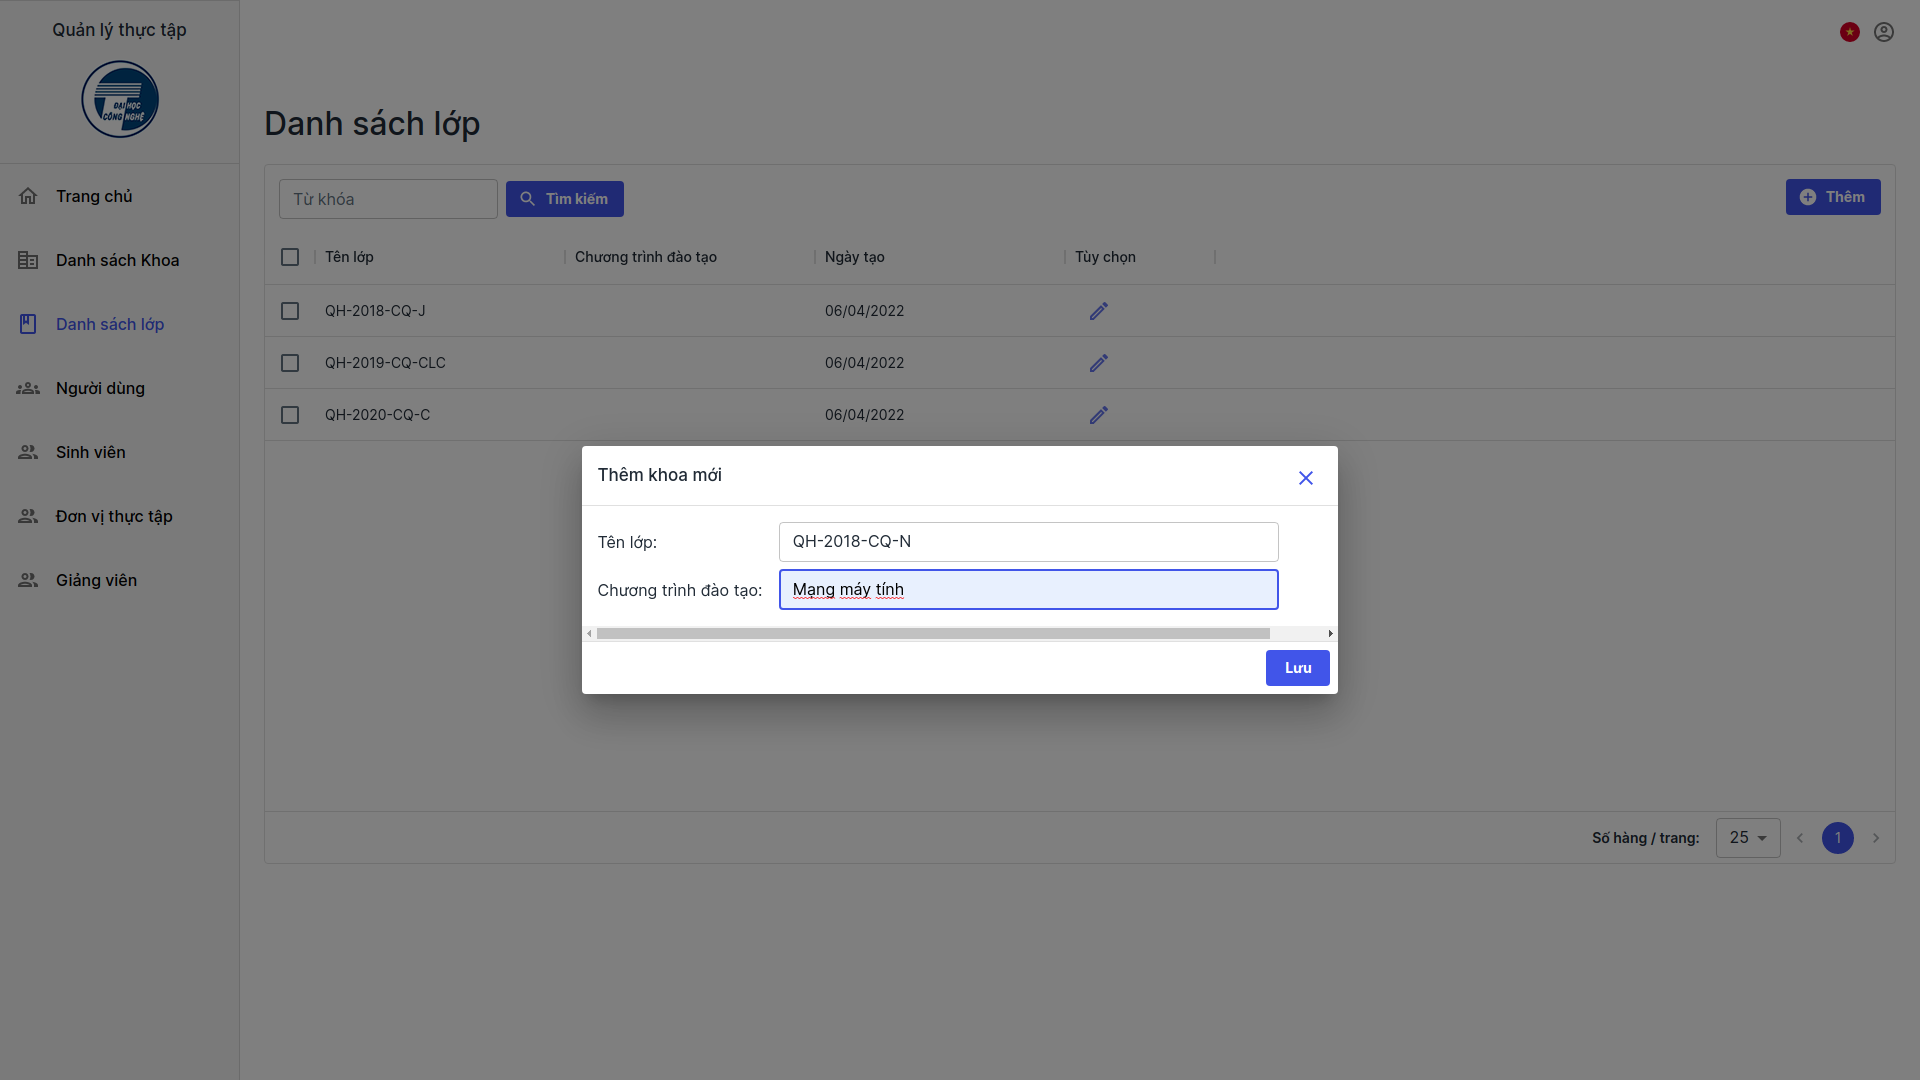
\includegraphics[width=\linewidth]{./images/image25.png}
	\caption{Màn hình tạo Lớp mới}
	\label{fig:add_class}
\end{figure}

\begin{figure}[]
	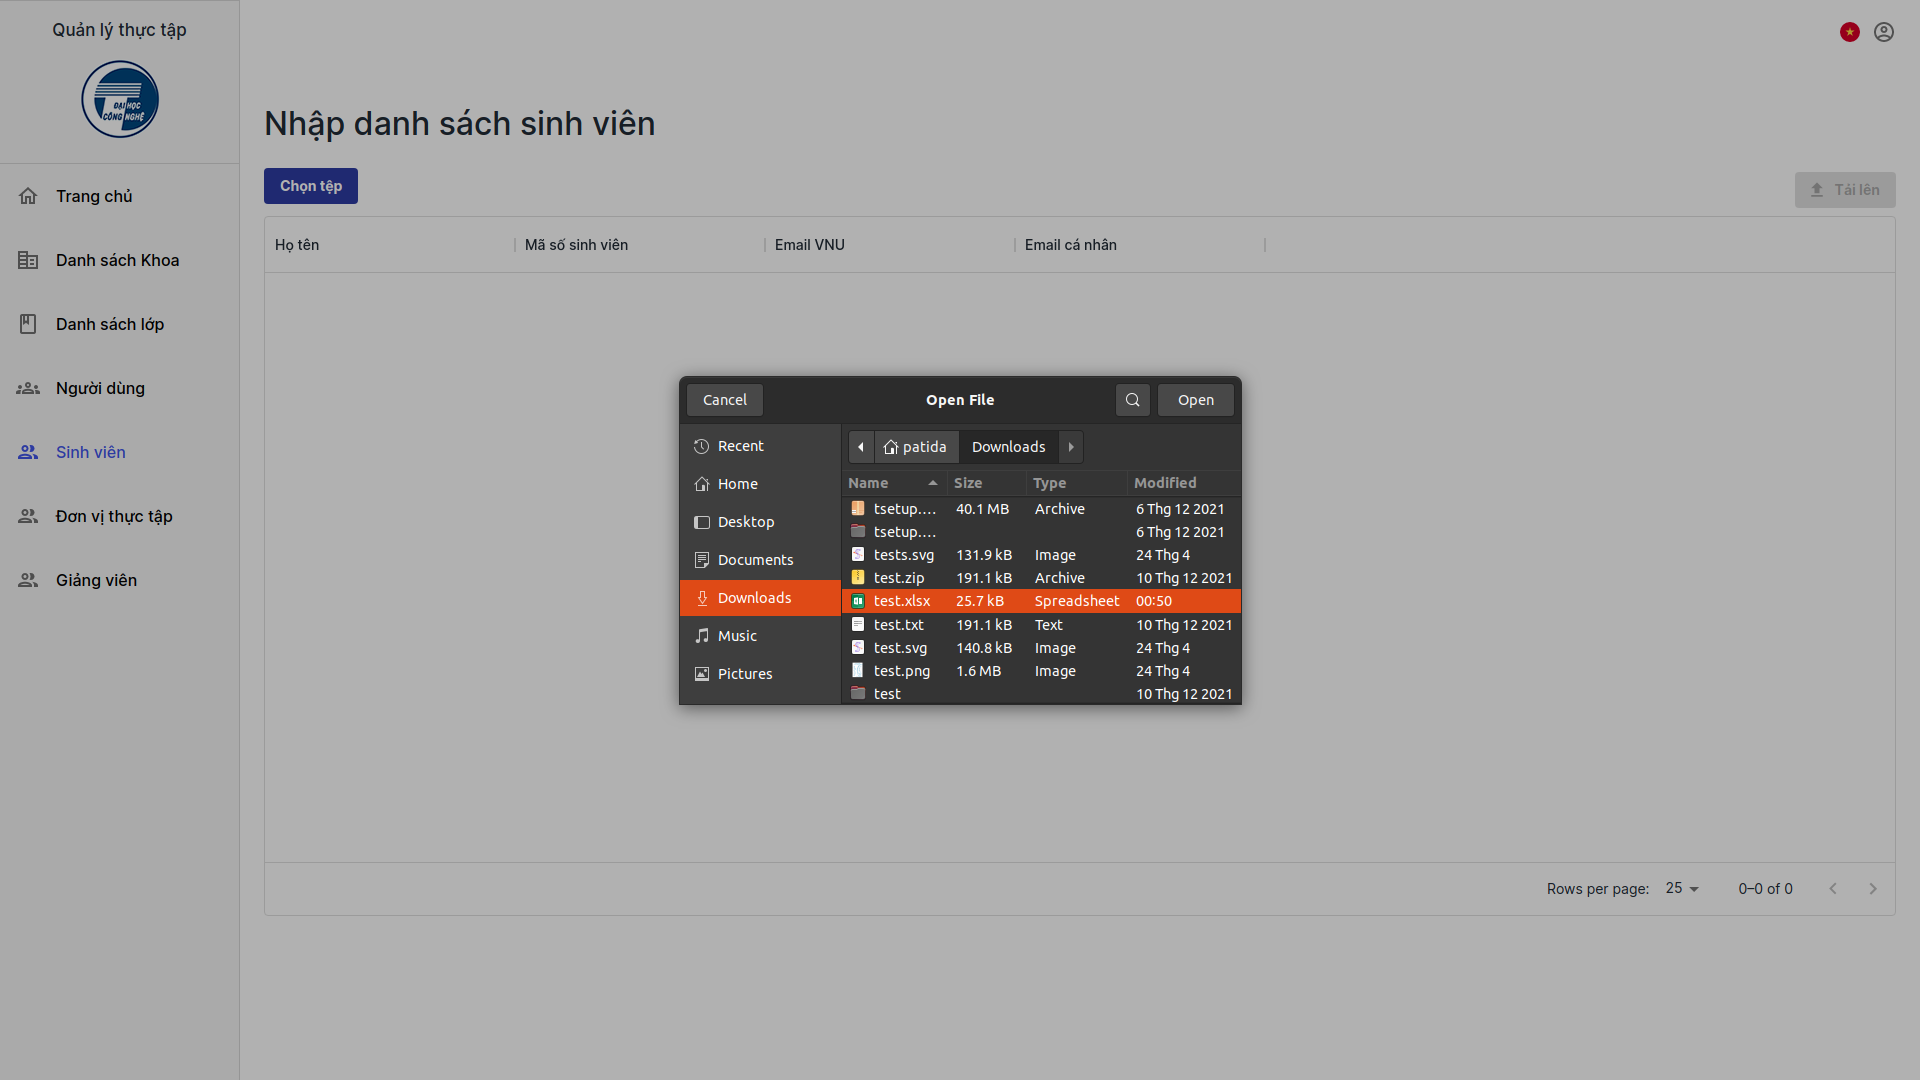
\includegraphics[width=\linewidth]{./images/image27.png}
	\caption{Màn hình chọn file Danh sách sinh viên}
	\label{fig:choose_file}
\end{figure}

\begin{figure}[]
	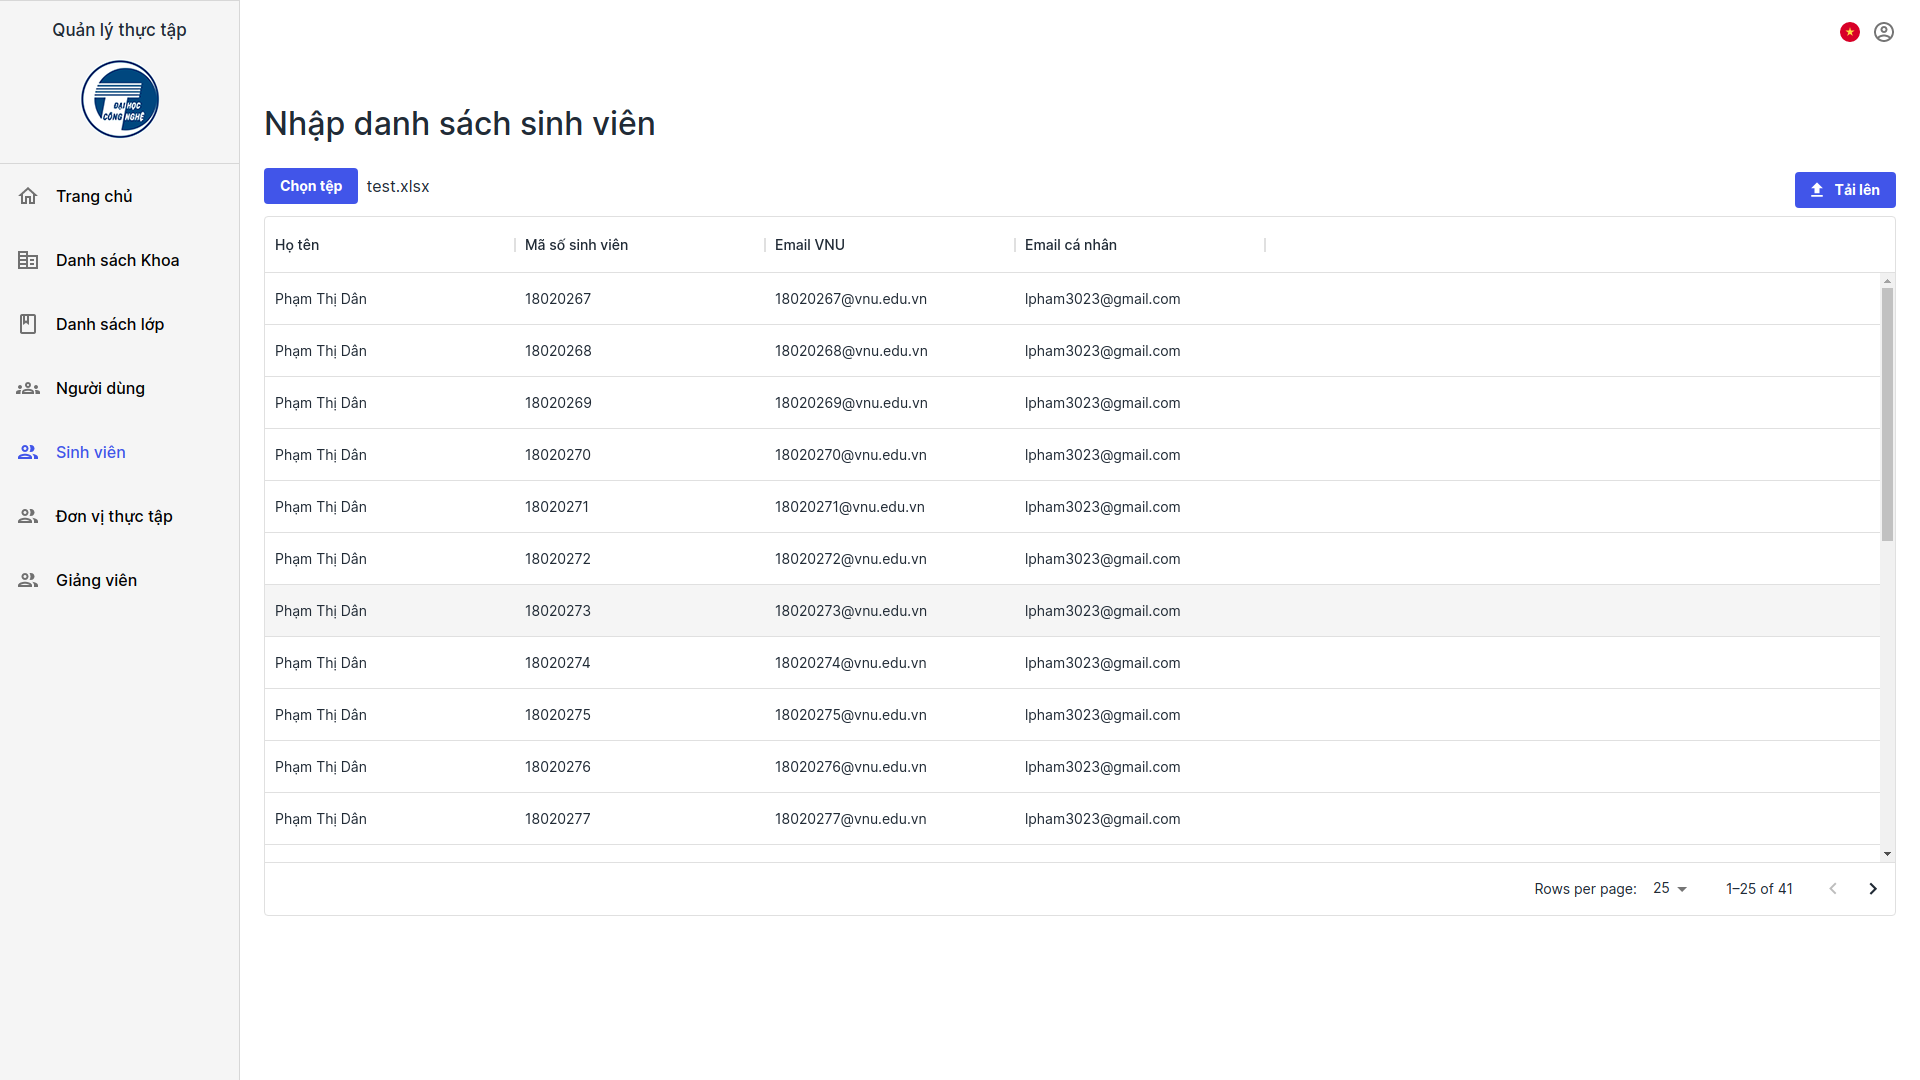
\includegraphics[width=\linewidth]{./images/image28.png}
	\caption{Màn hình tải lên file Danh sách sinh viên}
	\label{fig:upload_list}
\end{figure}

\end{document}